% Preamble
\documentclass [11pt]{article}

\usepackage{setspace}
\usepackage{amssymb}
\usepackage{amsmath}
\usepackage{amsfonts}
\usepackage{amssymb}
\usepackage{setspace}
\usepackage{amsthm}
\usepackage{textcomp}
\usepackage{graphicx}
\usepackage{url}
\usepackage{color}
\usepackage[dvipsnames]{xcolor}
\definecolor{cuteBlue}{rgb}{0.258, 0.387, 0.574}
\definecolor{cuteGreen}{rgb}{0, 0.3, 0}
\usepackage{cancel}
\usepackage{comment}
\usepackage[framemethod=TikZ]{mdframed}
\usepackage{enumitem}
\usepackage{wasysym}
\usepackage{listings}
\usepackage{float}
\usepackage{booktabs}
\usepackage{fixltx2e}
\usepackage{threeparttable}
\usepackage{titling}
\usepackage{zref-base}
\usepackage{makecell}
\usepackage{array}
\usepackage{hhline}
\usepackage{titlesec}
\usepackage{tcolorbox}

% To make jumping between equation, figure, citation references easier
\usepackage[colorlinks=true, urlcolor=cuteBlue, citecolor=cuteGreen, linkcolor=black]{hyperref}

% To make caption labels (i.e. Figure 1, Figure 2...) bold and
% make all caption text small
\usepackage[labelfont=bf, font=small]{caption}

% For strike-out text during editing
\usepackage[normalem]{ulem}

%Latin accents
\usepackage[utf8]{inputenc}

%subfigures
\usepackage{caption}

% Add author affiliations
\usepackage{authblk}

% %%%%%%%%%%%%%%%%%%%%%%%%%%%%%%%%%%%%%%%%%%%%%%%%%%%%%%%%%%%%%%%%%%%%%%%%%%%%%%
% %%%%%%%%%%%%%%%%%%%%%%%%%%%%%%%%%%%%%%%%%%%%%%%%%%%%%%%%%%%%%%%%%%%%%%%%%%%%%%

% Margins and spacings
\setlength{\evensidemargin}{0.0cm}
\setlength{\oddsidemargin}{0.0cm}
\setlength{\topmargin}{-1.0cm}
\setlength{\textwidth}{17cm}
\setlength{\textheight}{22cm}
\setlength{\parskip}{2.5mm}
\reversemarginpar
\marginparsep  0.1in
\marginparwidth 0.7in

% Give more spacing in equation arrays
\setlength{\jot}{10pt}

% Allow page breaks in multiline equations
\allowdisplaybreaks

% Set up title spacing so we don't waste so much space
\setlength{\droptitle}{-8em}
\date{\vspace{-5em}}  % No date will appear in title.

% Spacing between section headings and text
\titlespacing\section{0pt}{12pt plus 4pt minus 2pt}{-2pt plus 2pt minus 2pt}
\titlespacing\subsection{0pt}{12pt plus 4pt minus 2pt}{-2pt plus 2pt minus 2pt}
\titlespacing\subsubsection{0pt}{12pt plus 4pt minus 2pt}{-2pt plus 2pt minus 2pt}

% Convenient micron symbol
\newcommand{\micron}{{\textmu}m}

% No excess spacing for lists
\setlist{itemsep=0pt, topsep=0pt}

% Allow paragraph indentations in lists
\setitemize{listparindent=\parindent}
\setenumerate{listparindent=\parindent}

% Column type for tables with nice spacing
\newcolumntype{M}[1]{>{\centering\arraybackslash}m{#1}}
\newcolumntype{N}{@{}m{0pt}@{}}


% %%%%%%%%%%%%%%%%%%%%%%%%%%%%%%%%%%%%%%%%%%%%%%%%%%
% Document settings
% %%%%%%%%%%%%%%%%%%%%%%%%%%%%%%%%%%%%%%%%%%%%%%%%%%

% References
\usepackage[
	backend=bibtex,
	style=numeric-comp, % show references as [1-3] instead of [1,2,3]
	sorting=none,				% Do not sort bibliography
	url=false, 					% Do not show url in reference
	doi=false, 					% Do not show doi in reference
	isbn=false, 				% Do not show isbn link in reference
	eprint=false, 			% Do not show eprint link in reference
	maxbibnames=9, 			% Include up to 9 names in citation
]{biblatex}
% Add library
\addbibresource{./chann_cap_bib}

% Bold the 'Figure #' in the caption and separate it from the title/caption
% with a period
% Captions will be left justified
\usepackage[
	aboveskip=1pt,
	labelfont=bf,
	labelsep=period,
	justification=raggedright,
	singlelinecheck=off
]{caption}

% Add numbered lines
\usepackage{lineno}
\linenumbers

% Package to include multiple title pages
% This will allow me to add a tile to the main text and to the SI
\usepackage{titling}

% This package will allow me to define booleans to compile main text or SI
\usepackage{ifthen}
\newboolean{maintext}
\newboolean{sitext}

%%%%%%%%%%%%%%%%%%%%%%%%%%%%%%%%%%%%%%%%%%%%%%%%%%%%
% Personalized functions
%%%%%%%%%%%%%%%%%%%%%%%%%%%%%%%%%%%%%%%%%%%%%%%%%%%%
% Commenting
\newcommand{\mrm}[1]{\textcolor{cuteBlue}{(MR:~#1)}} % Commenting
\newcommand{\rp}[1]{\textcolor{red}{(RP:~#1)}} % Commenting
\newcommand{\note}[1]{\textcolor{ForestGreen}{(NOTE~#1)}} % Commenting

% To define more useful LaTeX commands
\usepackage{xparse}

% Equation referencing
\newcommand{\eref}[1]{Eq.~\ref{#1}}
% Figure referencing
\newcommand{\fref}[1]{Fig.~\ref{#1}}
% Table referencing
\newcommand{\tref}[1]{Table~\ref{#1}}
% Section referencing
\newcommand{\secref}[1]{Section~\ref{#1}}
% SI referencing
\newcommand{\siref}[1]{Appendix~\ref{#1}}

% Define command to begin the supplementary section
\newcommand{\beginsupplement}{
				\setcounter{section}{0} % Restart section counter
        \renewcommand{\thesection}{S\arabic{section}}%
        \setcounter{table}{0} % Restart table counter
        \renewcommand{\thetable}{S\arabic{table}}%
        \setcounter{figure}{0} % Restart figure counter
        \renewcommand{\thefigure}{S\arabic{figure}}%
        \setcounter{equation}{0} % Restart equation counter
        \renewcommand{\theequation}{S\arabic{equation}}%
     }

%%%%%%%%%%%%%%%%%%%%%%%%%%%%%%%%%%%%%%%%%%%%%%%%%%%%
% Personalized math functions
%%%%%%%%%%%%%%%%%%%%%%%%%%%%%%%%%%%%%%%%%%%%%%%%%%%%
% Vector P (for distribution vector)
\newcommand{\PP}{\bb{P}}
% Expected value
\newcommand{\ee}[1]{\left\langle #1 \right\rangle}
% Bold math
\newcommand{\bb}[1]{\mathbf{#1}}
% Time derivative
\newcommand{\dt}[1]{{d{#1} \over dt}}
\newcommand{\ddt}[1]{{\partial{#1} \over \partial t}}
% Time step
\newcommand{\Dt}{\Delta t}
% tot as in total number of organisms
\newcommand{\tot}{_{\text{tot}}}
% Euler's number e
\newcommand{\E}{\mathrm{e}}

% Specify i^th entry
\newcommand{\tth}{^{\text{th}}}

%%%%%%%%%%%%%%%%%%%%%%%%%%%%%%%%%%%%%%%%%%%%%%%%%%%%
%% Begin document
%%%%%%%%%%%%%%%%%%%%%%%%%%%%%%%%%%%%%%%%%%%%%%%%%%%%

\title{
\textbf{Statistical Genetics Notes}
}
% Authors
\author[1]{Manuel Razo-Mejia}
\author[1, 2, 3, *]{Rob Phillips}

% Affiliations
\affil[1]{Division of Biology and Biological Engineering, California Institute
of Technology, Pasadena, CA 91125, USA}
\affil[2]{Department of Physics, California Institute of Technology, Pasadena,
CA 91125, USA}
\affil[3]{Department of Applied Physics, California Institute of Technology,
Pasadena, CA 91125, USA}
\affil[*]{Correspondence: phillips@pboc.caltech.edu}

% date
% \date{\today}

\setcounter{Maxaffil}{0}
% Set affiliations in small font
\renewcommand\Affilfont{\itshape\small}

\begin{document}
%% MAIN TEXT
\maketitle % Set title for paper

\tableofcontents

% Chapter 1. Deterministic evolution
% % !TEX root = ../../main.tex
\section{Natural selection (survival of the fittest)}
\label{sec_selection}
1859 marked the year that Charles Darwin shocked the world with the incredible
insights contained in his book \textit{On the origin of Species}. The complete 
title of the book \textit{On the Origin of Species by Means of Natural
Selection, or the Preservation of Favoured Races in the Struggle for Life}
captures perfectly Darwin's proposed mechanism for how evolution takes place.
Nowadays with the so-called modern-synthesis of evolution we know that natural
selection is not the only evolutionary force that shapes living organisms. In
the coming sections we will mathematically explore mechanisms such as mutation
and genetic drift that all contribute to form the many \textit{endless forms,
most beautiful} that live in our planet. But we will begin with the first
evolutionary force discovered by Darwin and Alfred Russel Wallace.

Natural selection is intrinsically associated with the concept of fitness. The
phrase ``survival of the fittest'' first used by Darwin guided and still guides
the way that biologists think about the evolution of many organisms. But
despite the fact that fitness is part of the daily jargon of many biologists,
it is a subtle and highly debated concept. After all what defines the ability
of an organism to survive the challenges that surround them are completely
context dependent. Roughly speaking we can think of fitness as the ability of
an organism, or a population of organisms to survive and reproduce in the given
ecological niche they occupy. The term ecology has to be included because
fitness is a result of the interplay between organisms with their environment
including all biotic and abiotic interactions. 

It is common both in theory and in experiments to use the relative growth rates
of organisms, i.e. the speed at which they can reproduce and generate
offspring, as a proxy for fitness. This is a convenient approximation both
for experiments and for theory, but one should not lose track of the relevant
context dependence on the fitness. Just because redwoods have an average life
span of 500-700 years and a very low growth rate that doesn't mean they are not
fit. Having said that we will first begin with the simplest form of fitness,
i.e. frequency independent selection. The term frequency independence simply
refers to the assumption that the fitness of a particular allele does not
depend on the relative abundance of such allele. This assumption could break
down for cases such as some pathogenic bacteria that coordinate their attack
via cell-to-cell communication known as quorum sensing. But we need to learn
how to crawl before we try to run.

\subsubsection{Frequency independent selection (haploids)}

Because of our personal love for bacteria and the fact that many of the most
interesting experiments in evolution have been and are being done in haploid
organisms, we will first focus our efforts on these single-cell organisms.
Haploidy refers to the biological feature of having a single copy of a
chromosome. As bacteria divide into two cells they segregate (split) one copy
of the genome to each of the daughter cells (extrachromosomal elements such as
plasmids behave differently). This in contrast with diploidy where organisms
such as humans that receive one copy of each chromosome form each parent. What
haploidy means for our task of modeling selection on a one-locus two-allele
system is that we only need to focus on the fitness value of each of the
alleles without having to worry about combination of alleles.

For the simplest case of one-locus two-alleles let us define the two alleles to
be $A$ and $a$. Let $N_A(t)$ and $N_a(t)$ be the corresponding number of
organisms carrying each allele at time $t$. For the frequency-independent 
selection we have that the change in number of organisms with allele $A$ is of
the form
\begin{equation}
  \dt{N_A} = f_a N_A(t),
\end{equation}
where $f_a$ is the growth rate of organisms carrying this allele on a
particular fixed environment. As discussed before we will use this growing rate
as a proxy for fitness; this is sometimes called Malthusian fitness after
Thomas Robert Malthus, a famous scholar whose assay on population growth
inspired both Darwin and Wallace. We can define an equivalent equation for
allele $a$ with fitness $f_a$.

We are not particularly interested in tracking the absolute number of organisms
with a specific genotype, but their relative abundance. Therefore let us define
$N\tot(t) \equiv N_A(t) + N_a(t)$ and the relative abundance of allele $A$ as
\begin{equation}
  x(t) = {N_A(t) \over N\tot(t)}.
\end{equation}
The time dynamics for $N\tot(t)$ are of the form
\begin{equation}
  \dt{N\tot(t)} = \bar{f}(t) N\tot(t),
\end{equation}
where $\bar{f}(t)$ is the average fitness of the population at time $t$. We can
deduce the value of $\bar{f}(t)$ if we notice that the dynamics of the total
population is just the sum of the individual alleles dynamics, i.e.
\begin{equation}
  \dt{N\tot(t)} = \dt{N_A(t)} + \dt{N_a(t)} = f_a N_A(t) + f_a N_a(t).
\end{equation}
We can factorize an $N\tot(t)$ out of the equation and use the frequencies of
each allele to obtain
\begin{equation}
  \dt{N\tot(t)} = N\tot(t) \left[ f_a x(t) + f_a (1 - x(t)) \right].
\end{equation}
This shows us that the average fitness $\bar{f}(t)$ is of the form
\begin{equation}
  \bar{f}(t) = f_a x(t) + f_a (1 - x(t)).
\end{equation}

The dynamics that interest us are the dynamics of the allele frequency. We only
need to define the dynamics for one of the alleles since we are assuming a
two-allele model for which knowing the dynamics of one of them determines the
dynamics of the other. This looks like
\begin{equation}
  \dt{x} = \dt{}\left( {N_A(t) \over N\tot(t)} \right).
\end{equation}
Using the chain rule this gives
\begin{equation}
  \dt{x(t)} = {\dot{N}_A(t) N\tot(t) - N_A(t) \dot{N}\tot(t) \over N\tot(t)^2},
\end{equation}
where $\dot{N}_x = dN_x / dt$. Substituting the time derivatives gives
\begin{equation}
  \dt{x} = {[f_a N_A(t)] N\tot(t) \over N\tot(t)^2} -
           {N_A(t)[\bar{f}(t) N\tot(t)] \over N\tot(t)^2}.
\end{equation}
We now substitute the definition of the average fitness to obtain
\begin{equation}
  \dt{x} = {f_a N_A(t) - 
           N_A(t) [f_a x(t) + f_a (1 - x(t))]
          \over N\tot(t)},
\end{equation}
This can be further simplify by using the definition of the allele frequency to
obtain
\begin{equation}
  \dt{x} f_a x(t) - x(t)[f_a x(t) + f_a (1 - x(t))].
\end{equation}
Grouping terms by the fitness values results in
\begin{equation}
  \dt{x} = f_a x(t)(1 - x(t)) - f_a x(t)(1 - x(t))
  = s x(t)(1 - x(t)),
  \label{eq_freq_dynamics_selection}
\end{equation}
where we defined $s = f_a - f_a$, the fitness difference between both alleles,
also known as the selection coefficient. This differential equation is very
revealing; what it is telling us is that for there to be changes in the
population structure, i.e. for the population to evolve there needs to be a
fitness difference between the competing members of the population. For now
ignore that we are working under the unrealistic regime of unbounded
exponential growth, meaning that as the model is written, there is no upper
bound for how large a population could get. The central feature of
\eref{eq_freq_dynamics_selection} is that for there to be a change in the
composition of the population, which is what we define as evolution, the
fitness values for each mutant must differ. 

For the specific case that we are studying in which $s$ is a constant, meaning
that the fitness values of the alleles don't change over time we can solve this
differential equation. Specifically we can use the separation of variables
method to compute
\begin{equation}
  \int {dx \over x(1 - x)} = \int dt \;s,
  \label{eq_sep_var}
\end{equation}
where we drop the time dependence for notation convenience. For the left-hand
side of the equation we can use partial fractions and write
\begin{equation}
  {1 \over x(1 - x)} = {A \over x} + {B \over (1 - x)}
  = {A - Ax + Bx \over x(1 - x)}.
\end{equation}
For $A = 1$ and $B = 1$ we have
\begin{equation}
  {1 - x + x \over x(1 - x)} = {1 \over x(1 - x)}.
\end{equation}
This allows us to write \eref{eq_sep_var} as 
\begin{equation}
  \int {dx \over x} + \int {dx \over 1 - x} = s \int dt.
\end{equation}
Solving these integrals results in
\begin{equation}
  \ln x - \ln(1 - x) = \ln\left( {x \over 1 - x} \right) 
  = s t + C,
  \label{eq_sep_var_sol}
\end{equation}
where $C$ is an integration constant. If we set an initial condition $x(t = 0)
= x_o$ we find that
\begin{equation}
  C = \ln \left( {x_o \over 1 - x_o} \right).
\end{equation}
Substituting this value for $C$ and exponentiating both sides of
\eref{eq_sep_var_sol} gives
\begin{equation}
  {x \over 1 - x} = {x_o \over 1 - x_o} \E^{s t}
\end{equation}
Let's now solve for $x$. First we send the denominator on the left-hand side to
the other side
\begin{equation}
  x = (1 - x)\left( x_o \over 1 - x_o \right)\E^{st}
\end{equation}
Now we expand the product and send the terms with $x$ back to the left-hand
side
\begin{equation}
  x + x {x_o \over 1 - x_o}\E^{st} = {x_o \over 1 - x_o}\E^{st}.
\end{equation}
Factorizing $x$ results in
\begin{equation}
  x \left( 1 + {x_o \over 1 - x_o}\E^{st} \right) = {x_o \over 1 - x_o}\E^{st}.
\end{equation}
The term in parenthesis can be rewritten as
\begin{equation}
  x \left( {1 - x_o + x_o\E^{st} \over 1 - x_o} \right) =
  {x_o \over 1 - x_o}\E^{st}.
\end{equation}
This allows us to cancel the denominator on both sides of the equation to
obtain
\begin{equation}
  x \left[ 1 + x_o \left( \E^{st} - 1 \right) \right] = x_o \E^{st}.
\end{equation}
Finally we can solve for the allele frequency
\begin{equation}
  x = {x_o \E^{st} \over 1 + x_o \left( \E^{st} - 1 \right)}.
\end{equation}
This is the solution of the logistic equation. \fref{fig_01_01} shows this
solution for different selection coefficients. We can se that in this
deterministic regime as long as there is a fitness difference, i.e. as long as
$s \neq 0$, the fate of the population is set. If $s > 0$ allele $A$ will go
into fixation. Otherwise if $s < 0$ the allele will go extinct.

\begin{figure}[h!]
	\centering 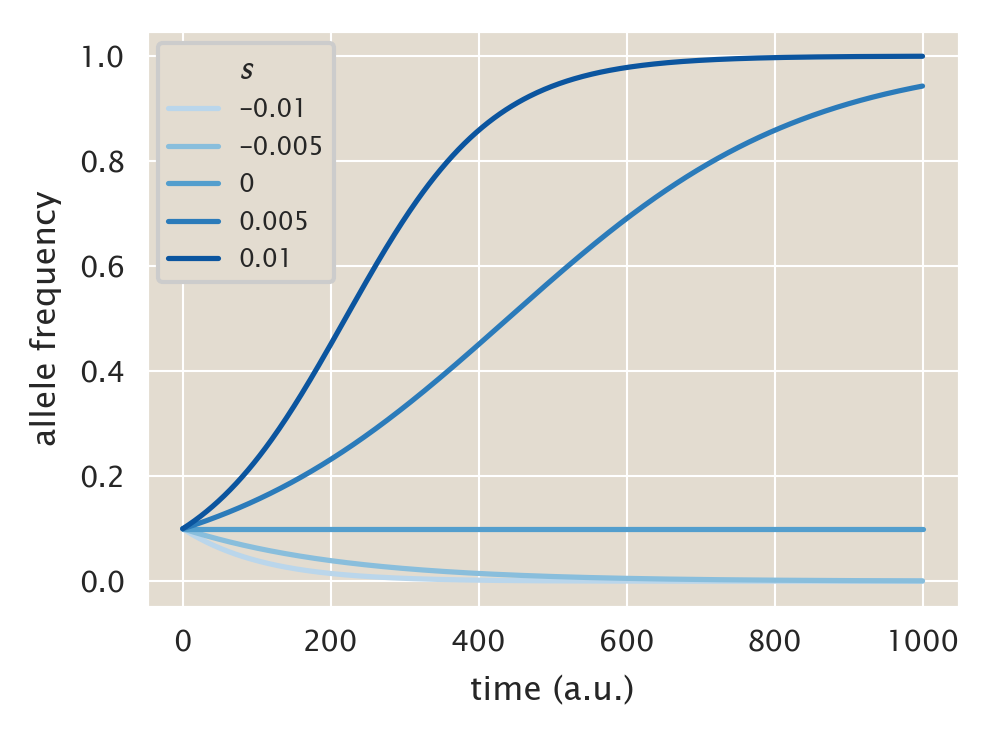
\includegraphics
  {../fig/deterministic_evo/01_01_deterministic_select.png}
  \caption{\textbf{Allele frequency for deterministic selection}. The 
	different curves show allele frequency dynamics for a one-locus two-allele
	system. The fate of the allele is determined by the value of the selection
	coefficient, but the speed to fixation depends both on the initial allele
	frequency and on the magnitude of the selection coefficient.}
  \label{fig_01_01}
\end{figure}
% % !TEX root = ../../main.tex
\subsection{Mutation}\label{seq_determ_mut}

One of the ingredients for evolution to take place is the constant appearance
of genetic variability. After all, the raw material for evolution to act on is
the appearance of new mutations in the population. This is what we will model
now for our one-locus two-allele case. We will think of mutations between both
alleles $A$ and $a$ as a simple first-order chemical reaction of the form
\begin{equation}
  A \xrightleftharpoons[\mu_{a A}]
  {\,\mu_{A a}\,} a,
\end{equation}
where $\mu_{A a}$ is the mutation rate from $A$ to $a$ and 
$\mu_{a A}$ is the mutation rate from $a$ to $A$. A useful way to
interpret the mutation rate is as the probability of switching allele per unit
time. That means that on a small time window $\Dt$ a single organism has a
probability of switching from $A$ to $a$ of
\begin{equation}
  P(A \rightarrow a \mid \Dt) = \mu_{A a} \Dt, \quad 
  \text{for } \Dt \ll \mu_{Aa}.
\end{equation}
What this implies is that for this small time window every organism carrying
allele $A$ flips a coin with probability $\mu_{A a} \Dt$ of getting
heads. If the outcome of the coin is indeed heads, the allele is mutated,
otherwise it remains the same. So when writing a differential equation to model
this phenomena we must multiply the number of organisms by the mutation rate.
This results in a differential equation for the change in number of organisms
carrying $A$ of the form
\begin{equation}
  \dt{N_A} = 
  \underbrace{- \mu_{A a} N_A(t)}_{\text{loss } A \rightarrow a}
  \underbrace{- \mu_{a A} N_a(t)}_{\text{gain } a \rightarrow A},
\end{equation}
where, as indicated, we must account for number of organisms that ``exit'' the
$A$ allele state by mutating to $a$, and the number of organisms that ``enter''
the state by mutating from $a$ to $A$. We can write an equivalent equation for
$N_a$ where the signs would be simply flipped since every time an organism is
lost from allele $A$ it must be gained in allele $a$, and vice versa. This
implies that for this case where there is only mutation $N\tot$ does not change
over time since the number of organisms is assumed to be conserved.

Let us now write the dynamics that we actually care about, that is the allele
frequency $x(t)$. This takes the form
\begin{equation}
  \dt{x} = \dt{}\left( {N_A \over N\tot} \right) = {1 \over N\tot} \dt{N_A},
\end{equation}
where we took $N\tot$ out of the derivative since for this case we said it
doesn't change over time. Substituting the dynamics of $N_A$ and using the
definition of the allele frequency we obtain
\begin{equation}
  \dt{x} = - \mu_{A a} x + \mu_{a A} (1 - x),
  \label{eq_mutation_ode}
\end{equation}
where we again suppressed the time dependence for notation simplicity. This
equation can also be solved analytically, but before getting to that solution
let's take a look at the steady state value. After all we know that these are
deterministic dynamics so the allele fraction will reach a unique point. The
steady state results in
\begin{equation}
  \mu_{A a} x_{ss} = \mu_{a A} (1 - x_{ss}),
\end{equation}
where $x_{ss}$ indicates that it is the steady state allele frequency. If we
now solve for $x_{ss}$ this results in
\begin{equation}
  x = {\mu_{a A} \over \mu_{a A} + \mu_{A a}}.
\end{equation}
So the equilibrium allele frequency for this case is given by the rate of how
often strains mutate from $a$ to $A$ divided by the sum of those rates. That
means that in the limit where it is much more likely to mutate from $a$ to $A$,
i.e. $\mu_{a A} \gg \mu_{A a}$ the allele frequency goes
to one, i.e. allele $A$ will go into fixation. The opposite would be true for a
much larger mutation rate from $A$ to $a$.

Now let's go ahead and solve the actual dynamics. \eref{eq_mutation_ode} is an
ordinary differential equation that can again be solved by separation of
variables. This is
\begin{equation}
  \int {dx \over - \mu_{A a} x + \mu_{a A} (1 - x)} = 
  \int dt.
\end{equation}
Evaluating the integrals results in
\begin{equation}
  -{1 \over \mu_{a A} + \mu_{A a}}
  \ln \left( \mu_{A a} x - \mu_{a A} (1 - x) \right) =
  t + C,
  \label{eq_mutation_int}
\end{equation}
where $C$ is an integration constant. Using again the initial condition where
$x(t=0) = x_o$ we have that
\begin{equation}
  C =  -{1 \over \mu_{a A} + \mu_{A a}}
  \ln \left( \mu_{A a} x_o - \mu_{a A} (1 - x_o) \right).
\end{equation}
Using this result we can rewrite \eref{eq_mutation_int} as
\begin{equation}
  -{1 \over \mu_{a A} + \mu_{A a}}
  \ln \left( { \mu_{A a} x - \mu_{a A} (1 - x)
    \over
  \mu_{A a} x_o - \mu_{a A} (1 - x_o)} \right) = t.
\end{equation}
Exponentiating both sides gives
\begin{equation}
  \left( { \mu_{A a} x - \mu_{a A} (1 - x)
    \over
  \mu_{A a} x_o - \mu_{a A} (1 - x_o)} \right)^{
    -{1 \over \mu_{a A} + \mu_{A a}}} = \E^t
\end{equation}
If we now elevate both sides to the $\mu_{a A} + \mu_{A\rightarrow
a}$ power we obtain
\begin{equation}
  \left( { \mu_{A a} x - \mu_{a A} (1 - x)
    \over
  \mu_{A a} x_o - \mu_{a A} (1 - x_o)} \right) =
  \E^{- (\mu_{a A} + \mu_{A a}) t}.
\end{equation}
We can now solve for $x$ and after a little bit of algebra we find that
\begin{equation}
  x(t) = {\mu_{a A} 
  \over 
  \mu_{a A} + \mu_{A a}} -
  {\left[  
  \mu_{a A} -
  (\mu_{a A} + \mu_{A a}) x_o
  \right] 
  \E^{- (\mu_{a A} + \mu_{A a}) t}.
  \over
  \mu_{a A} + \mu_{A a}}.
\end{equation}
A little tricky solution, but we can easily see that in the limit when $t
\rightarrow \infty$ the second term on the right hand side goes to zero,
leaving behind the steady state solution we found before.
\fref{fig_deterministic_mut} shows the dynamics for different ratios of the
mutation rates. We can see that as expected the allele frequency converges to
the steady state value we derived.

\begin{figure}[h!]
	\centering 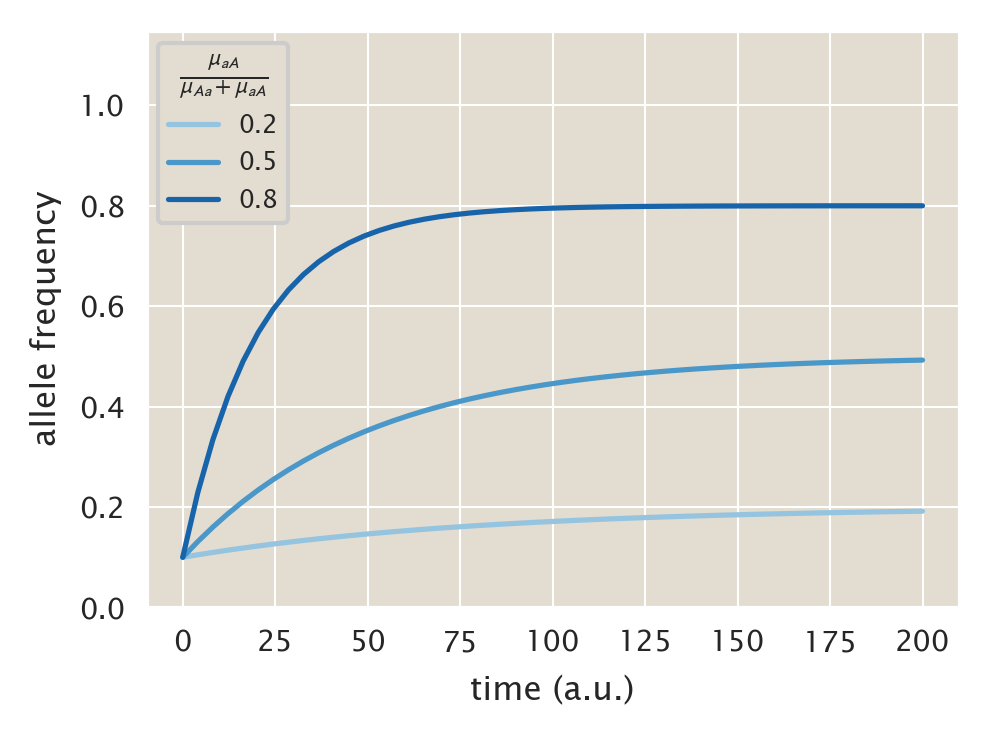
\includegraphics
  {../../fig/deterministic_evo/01_02_01_deterministic_mut.png}
	\caption{\textbf{Allele frequency for mutation only}. The different curves
	show allele frequency dynamics for a one-locus two-allele system mutating
	between both alleles. The steady state allele frequency is set by the ratio
	of the mutation rates.}
  \label{fig_deterministic_mut}
\end{figure}

\subsubsection{Mutation-Selection Balance}

Now that we have modeled two of the three forces we will be using throughout
the notes let us try to put them together. Since both selection and mutation
are directional deterministic forces we can easily add them together for our
allele frequency dynamics and still obtain a deterministic answer. The dynamics
for our single-locus two-allele system subject to both selection and mutation
are given by the sum of the dynamics for each case. This is
\begin{equation}
  \dt{x} = s x (1 - x) - \mu_{Aa} x + \mu_{aA} (1 - x).
  \label{eq_sel_mut}
\end{equation}
This linear ODE can be solved analytically as you can asses yourself by plugin
this equation into a symbolic math package such as Mathematica or Sympy. The
problem is that the solution is not intuitive with a bunch of tangents and
arctangents that make it very difficult to look at. Nevertheless we can still
gain intuition from \eref{eq_sel_mut}. An interesting setting to analyze is the
case where one of the alleles, let's say $a$ is deleterious, i.e. $s < 0$. If
that were the case our results from \secref{sec_selection} tell us that natural
selection would remove this allele from the population. But if mutation keeps
bringing the allele back over and over again, there should be a balance between
mutation and selection. This is a plausible scenario if we think of allele $A$
as a functional protein, and $a$ is a coarse-grained state of all
non-functional proteins for example. To compute this equilibrium we need to
compute the steady state for \eref{eq_sel_mut} as
\begin{equation}
  0 = s x_{ss}^2 + (\mu_{Aa} + \mu_{aA} - s) x_{ss} - \mu_{aA},
\end{equation}
where we already expanded the terms and group by powers of $x_ss$, the steady
state allele frequency. The roots of this quadratic equation are given by
\begin{equation}
  x_{ss} = {(s - \mu_{Aa} - \mu_{aA}) \pm 
    \sqrt{(\mu_{Aa} - \mu_{aA} - s)^2 + 4 s \mu_{aA}}
    \over 2s}.
\end{equation}
If again we take $a$ as a coarse-grained state for a non-functional gene we can
assume that reversing the mutation to the functional allele is very unlikely,
therefore we can set $\mu_{aA} \approx 0$. This results in
\begin{equation}
  x_{ss} = {(s - \mu_{Aa}) \mp (s - \mu_{Aa}) \over 2s}.
\end{equation}
The resulting two possible steady states are then
\begin{equation}
  x_{ss1} = 0, \quad x_{ss2} = 1 - {\mu_{Aa} \over s}.
\end{equation}
The first case shows that if allele $A$ were to go extinct it would stay as
such. The more interesting and relevant case is the second root. This shows
that the allele frequency decreases from the fixation value 1 depending on the
relative strengths of mutation and selection.

% Chapter 2. Introduction to Langevin equation
% !TEX root = ../../main.tex
\section{Genetic drift and the stochastic nature of evolution}

So far we have studied two of the forces of evolution from a deterministic
perspective. This sounds contradictory given the intuition that biologists have
about how the evolutionary process works. On the one hand any biologist will
tell you that evolution is a completely random process; from the emergence of a
beneficial mutation to the process of fixing this mutation in the population,
these dynamics are hard if not impossible to predict.

On the other hand in a conflicting view of evolution, biologists tend to
associate every biological feature to a product of selection. Either natural or
sexual selection, the literature is full of ``just-so-stories'' that attribute
a functional purpose to every aspect of biological systems. Therefore the claim
is that the process occurs at random, but everything serves a purpose. The
truth most likely lies somewhere in between.

At the dawn of the modern synthesis of evolutionary theory Sewall Wright came
to the conclusion that reproductive stochasticity could play an important role
in the fate of populations. In other words, not because a beneficial mutation
appeared in the population it would necessarily take over the population.
Accidents in evolution still play an important role when it comes to setting
the fate of a population. From a beneficial mutation being lost due to some
non-selection related event such as a stochastic death of the organism carrying
the mutation, to the fixation of deleterious mutations in the population. As a
matter of fact one of Sewall Wright's own students designed a beautiful
experiment to test these ideas on evolution.

\subsection{The Buri experiment}

\mrm{This section will probably live in the discrete evolution part of the 
notes once they exist. But for now I want to use Buri to motivate the reason
for thinking about drift. It doesn't necessarily fit with the bacteria-centered
tone of the notes, but it is such a great experiment!}

In 1956 Peter Buri, a student of Sewall Wright published the now classic paper
``\textit{Gene Frequency in Small Populations of Mutant Drosophila}'' in which
he experimentally demonstrated the concept of genetic drift.  The idea for this
beautiful experiment is depicted in \fref{fig_02_buri_schematic}. Briefly, Buri
began with eight female and eight male flies, all heterozygotes of the
\textit{bw} locus. This means that all of the flies had 1 copy of the gene
associated with white eyes, and one copy of the gene associated with  red eyes.
The phenotype that this combination of alleles gives is flies with orange eyes.
He then allowed the flies to reproduce, and after removing the adults, he
randomly chose 8 males and females from the next generation of offspring
without looking at the eye color. These new 8 males and 8 females were
transferred to a new flask and the procedure was repeated for 19 generations.

\begin{figure}[h!]
\centering 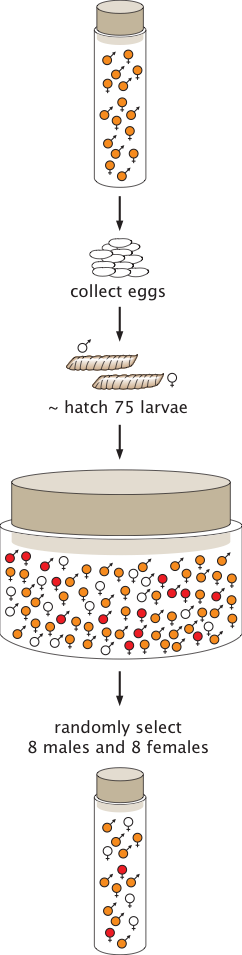
\includegraphics[scale=0.8]
  {../fig/drift_langevin/02_buri_schematic.png}
  \caption{\textbf{Buri's experimental setup.} At time $t=0$ eight
  heterozygote females and eight heterozygote males were allowed to reproduce.
  From their offspring, eight males and eight females were chosen at random and
  transferred into a new flask.}
  \label{fig_02_buri_schematic}
\end{figure}

Since the offspring that made it to the next generation were chosen at random,
Buri knew that the outcome would be different if he repeated an identical
experiment in different vials. As a result, for statistical power he
simultaneously tracked 107 flasks as shown in \fref[figBuriSchematic]. Each
generation, he counted the number of red-eyed, white-eyed and orange-eyed flies
he had randomly chosen. \fref[figBuriGenerations] shows the outcomes for these
different vials after 19 generations. Because the flies are allegedly mating at
random, with each generation there is an accumulation of fluctuations. As a
result, after 19 generations, many vials contained only white-eyed or red-eyed
flies, though some vials still contained a mixture of eye colors.

\begin{figure}[h!]
\centering 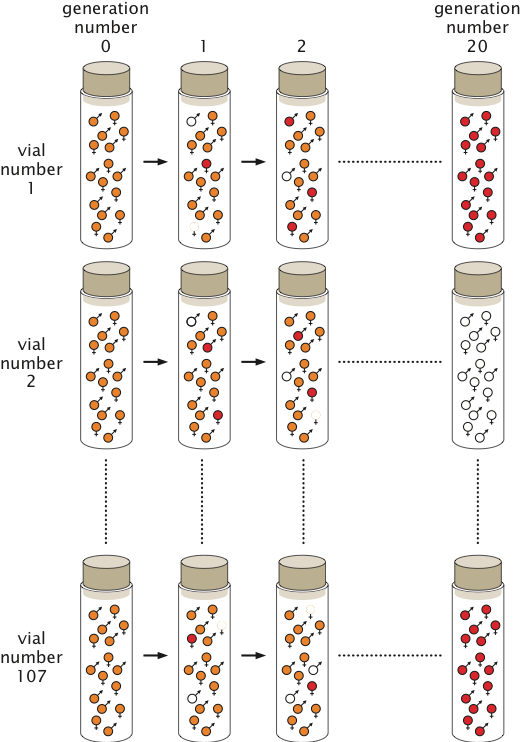
\includegraphics[scale=0.7]
  {../fig/drift_langevin/02_buri_generations.png}
  \caption{\textbf{Multiple replicates of the Buri experiment.}  Buri repeated
  his experiment in 107 separate vials, with the evolutionary trajectory
  different each time as a result of genetic drift.  Note that in the long time
  limit, many of the vials have gone to fixation with all flies having either
  white or red eyes.}
\label{fig_02_buri_generations}
\end{figure}

Having quantified the number of red-eyed, white-eyed and orange-eyed flies Buri
was able to quantify the frequency of alleles in the population. Since none of
the alleles were dominant, he could infer the genotype  by looking at the
phenotype of the flies.

\fref{fig_02_buri_experiment} summarizes the results of the experiment. By
tracking alleles over time with these 107 populations exposed to the same
conditions, Buri was able to observe evolution driven entirely by genetic
drift! He saw how in some of the populations one of the alleles went extinct,
arising from nothing more than the fluctuations inherent in small populations.

\begin{figure}[h!]
\centering
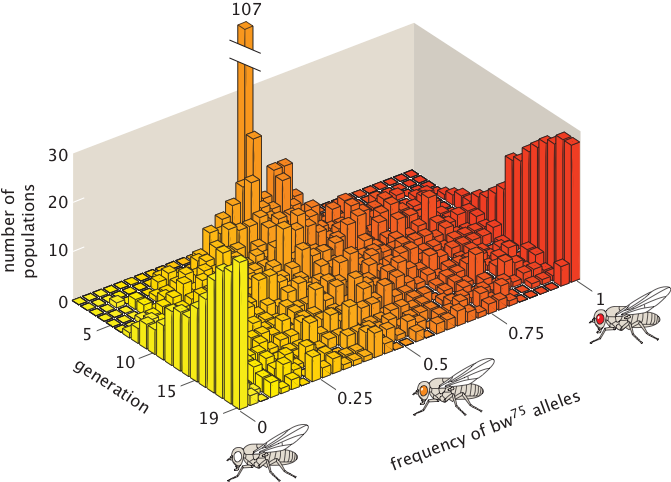
\includegraphics[scale=0.85]
  {../fig/drift_langevin/02_buri_experiment.png}
  \caption{\textbf{Results of the Buri experiment.} By tracking the phenotypes
  of the  flies, Buri was able to infer the allele frequencies for each
  population. The allele frequencies change as a result of genetic drift and
  after 19 generations, many of the vials contain flies all with the same eye
  color, implying fixation of alleles and evolution due to genetic drift.}
  \label{fig_02_buri_experiment}
\end{figure}

Now that we have looked at an experimental evidence of genetic drift on a
laboratory experiment let's go back to the mathematical modeling of this phenomena.
\subsection{Stochastic process}

When describing how a quantity evolves over time with a non-deterministic
trajectory we often use what is commonly known as stochastic processes. For
example imagine we are keeping track of a random variable $X$ that changes over
time. This stochastic variable $X$ could describe things such as count of a
specific chemical species, average price of an asset over a period of time,
frequency of a particular allele on a population, etc. To describe how this
variable $X$ changes over time we could in principle list an infinite number of
functions
\begin{equation}
  X(t) = f(X, t).
\end{equation}
This is what we call a stochastic process, i.e. the time evolution of a random
variable $X$. What we are doing here is considered notation abuse by the more
scrupulous mathematicians. Usually people prefer to define a random process as
$Y_X(t) \equiv f(X, t)$ to specify that we are studying how a random variable
$X$ evolves over time $t$ without compromising the use of $X$ as the sole
random variable, but I personally find that notation too strict. Most of our
efforts in these notes will go into describing the probability distribution of
such processes $P(x, t)$, i.e. the probability of our particular random process
taking the specific value $X(t) = x(t)$. More on that later.

Let's clarify all these subtle but important notation differences: The random
variable $X$ is a mapping from a random event to the real line; in other words,
for a particular quantity that we want to describe we assign a number to
represent the event that happened. A useful example is to think about it as
getting to observe a specific face once we roll a die, and assigning a number
from 1 to 6 to represent the face we observed. The stochastic process $X(t)$
describes the values that our random variable $X$ can take over time. Following
up with the die example this could be rolling a die every so often and keeping
track of the numbers that we obtain. This process $X(t)$ represents the
\textbf{ensemble} of possible realizations $x(t)$. In other words, as shown
schematically in \fref{fig02_02_01} $X(t)$ describes all possible values that
the quantity $X$ can take over time, and $x(t)$ describes a specific trajectory
that happened to occur for a specific realization of the process.

\begin{figure}[h!]
	\centering 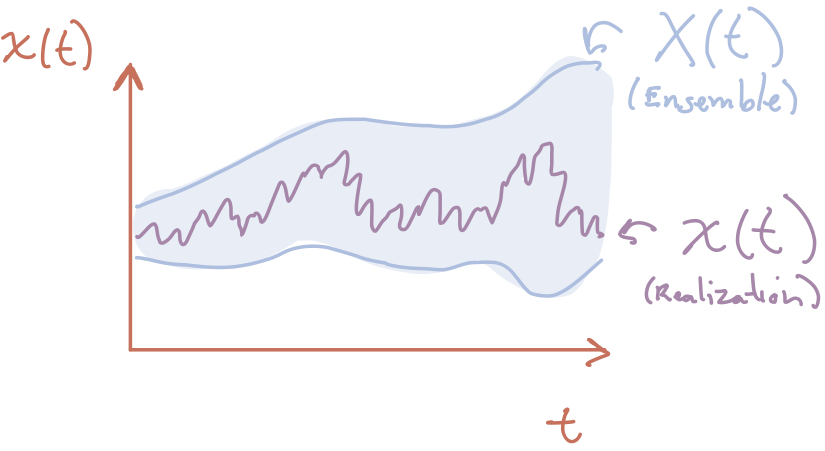
\includegraphics[width=0.5\textwidth]
  {../fig/drift_langevin/02_02_01_ensemble_realization.jpeg}
	\caption{\textbf{Schematic description of a stochastic process}. The shaded
	region describes the stochastic process $X(t)$, i.e. all the possible values
	that the random variable $X$ can take over time. The particular realization
	$x(t)$ describes a specific trajectory that the random variable $X$ took in
	one particular case.}
  \label{fig02_02_01}
\end{figure}

From the intuition presented in \fref{fig02_02_01} we understand that all
possible trajectories that our stochastic process can take are contained in the
function $X(t)$. But some particular paths $x(t)$ are more likely to happen
than others. This is what the language of probability theory allows us to
compute! In principle we are interested in writing how likely it is for our
process to take a specific value $x(t)$. This is described by the probability
function $P(x, t)$ which will be at the center of our endeavors for these
notes. Once we define our stochastic process we might want to compute a moment
of the distribution. Recall that for a continuous random variable $X$ with
probability density function $P_X(x)$, a moment is defined as
\begin{equation}
  \ee{X^m} \equiv \int dx \; x^m P_X(x),
\end{equation}
where the integral is taken over all the values that $X$ can take. Notice that
our notation for the distribution $P_X(x)$ highlights that we are only
considering values that $X$ can take, no time involved so far. For our case
in which the random variable can change over time what we have to do is settle
for a specific time point $t^*$ and compute the average at that time point
\begin{equation}
  \ee{X(t^*)^m} \equiv \int dx \; x^m P(x, t^*).
  \label{eq_process_moment}
\end{equation}
Notice that this is still not making a statement about the time evolution of
our variable $X$, but rather committing to a specific time point $t^*$ and then
computing the $m\tth$ moment at that time point. An intuitive way to think
about this is to take a frequentist approach for probability. We imagine that
we get to observe many many individual trajectories $\{x_1(t), \ldots
x_n(t)\}$, as schematically shown in \fref{fig02_02_02} then what
\eref{eq_process_moment} is doing is computing the moment at a specific time
point $t^*$ highlighted also in \fref{fig02_02_02}.

\begin{figure}[h!]
	\centering 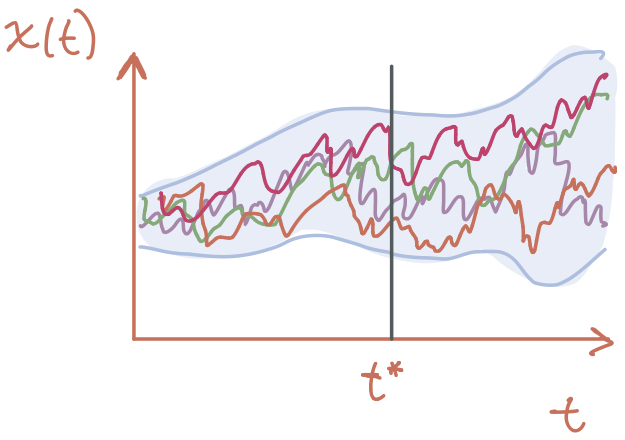
\includegraphics[width=0.5\textwidth]
  {../fig/drift_langevin/02_02_02_average_langevin.jpeg}
	\caption{\textbf{Computing a moment of a distribution $\ee{X(t)}$}. Multiple
  realizations of the stochastic process $\{x_1(t), \ldots x_n(t)\}$ are
  highlighted. In the limit where we have many many of these trajectories we
  can then compute a moment of the distribution $P(x, t^*)$ for a specific time
  point $t^*$. \mrm{need better caption}}
  \label{fig02_02_02}
\end{figure}

There is no reason why we have to limit ourselves to a single time point $t^*$.
In particular there are interesting quantities such as the autocorrelation
function $\kappa(t_1, t_2)$ that analyze how two different time points $t_1$
and $t_2$ covary with each other. This quantity is defined as
\begin{equation}
  \kappa(t_1, t_2) = \ee{\left(X(t_1) - \ee{X(t_1)}\right)
                         \left(X(t_2) - \ee{X(t_2)}\right)}.
\end{equation}
\mrm{Not sure if I will need to include this if we don't ge to compute moments
that refer to multiple time points.}

Having understood conceptually what stochastic process are and what they allow
us to do we are ready to see their practical implementation. The stochastic
process literature is rich and very formal, but it can be daunting to grasp the
basics of it. For our purposes we will take a more pragmatic approach rather
than diving into the intricacies of the formalism. Our fundamental equation to
model stochastic processes will be the Langevin equation.

\subsection{The Langevin equation}\label{sec_langevin_intro}

Since Robert Brown systematically described the jiggling of particles of
organic and inorganic origin under the microscope, physicists of the caliber of
Einstein and Smoluchowski tried to describe the phenomena. The first success
came from Einstein himself who in 1905 published a microscopic description of
Brownian motion at the time where the atomic structure of matter was still up
in the air. In 1908 only three years later, motivated by this theoretical
predictions, Jean Baptiste Perrin experimentally confirmed Einstein's theory to
unambiguously settle the controversy behind the existence of atoms. That same
year Paul Langevin published a seminal paper in which he proposed an
``infinitely simpler'' formulation of Brownian dynamics according to himself.
In doing so Langevin made use of what we know nowadays as a stochastic
differential equation. Ever since, the study of microscopic particles jiggling
under thermal forces has had enormous consequences in our understanding of the
structure of matter, and has motivated the development of the mathematical
formalism of stochastic calculus with great impact in physics, economics, and
as we are concerned here biological evolution.

The mathematical object that Langevin proposed that now carries his name is
different form the standard ordinary differential equations in the sense that
it includes a stochastic term. More specifically for a 1D system the Langevin
equation that describes the dynamics of $x(t)$ is of the form
\begin{equation}
  \dt{x} = A(x, t) + B(x, t) \xi(t),
  \label{eq_langevin}
\end{equation}
where $A(x, t)$ is the directional deterministic field that could depend on the
variable $x$ itself as well as time, $B(x, t)$ is the scale associated with the
stochasticity of the process and $\xi(t)$ is the random variable associated
with the dynamics of $x(t)$. Without the second term on the right-hand side we
have a regular differential equation for which there is most likely a method to
solve it given that $A(x, t)$ is a well behaved function. The solution of 
\eref{eq_langevin} without this second term would be of the form
\begin{equation}
  x(t) = x_o + \int_{t_o}^t dt\; A(x, t),
\end{equation}
where $x_o$ is the initial condition, i.e. $x(t = t_o) = x_o$. This solution
would be a smooth deterministic trajectory for $x(t)$. The extra element that
makes \eref{eq_langevin} special is the stochastic term $B(x, t) \xi(t)$. 
$B(x, t)$ is simply a coefficient that determines the amplitude of the noise,
i.e. it sets the scale for how noisy the stochastic process $x(t)$ must be. But
the true innovative feature of \eref{eq_langevin} is $\xi(t)$, sometimes called
white noise. This term is itself a random variable, meaning that it is defined
by a probability distribution $P(\xi, t)$. The reason this term is called white
noise is because the noise is assumed to have mean zero, i.e. fluctuations that
randomly increase the value of $x(t)$ cancel with fluctuations that tend to
decrease $x(t)$ on average. This is mathematically expressed as
\begin{equation}
  \ee{\xi(t)} = 0.
\end{equation}
The second reason this term is called white noise is because the noise at time
$t$ is independent of the noise at any other point in time $t'$. This is
sometimes referred as delta-correlated noise because the way we express this
lack of time correlation between time points is through a $\delta$-function as
\begin{equation}
  \ee{\xi(t) \xi(t')} = 2D \delta(t - t'),
  \label{eq_noise_delta}
\end{equation}
where the prefactor $2D$ is put to resemble the origins of this equation where
$D$ represented the diffusion coefficient of the Brownian particle. What 
\eref{eq_noise_delta} is saying is that only when $t = t'$ the noise
autocorrelation function takes the magnitude $2D$ - that's what the 
$\delta$-function role is. In other words, independently of what the noise
magnitude was at time $t'$, the noise at time $t$ is sampled from a
distribution with mean $\ee{\xi(t)} = 0$ and variance $\ee{\xi(t)^2} = 2D$.

Since we are characterizing the noise via only its first two moments, i.e. the
noise and the variance, we take the distribution of $\xi(t)$ to be Gaussian.
This assumption is justified because of the central limit theorem that tells us
that the distribution of the sum of many independent random variables tends to
a Gaussian distribution. That means the the probability density function of
$\xi(t)$ is of the form
\begin{equation}
  P(\xi(t)) = {1 \over \sqrt{4 \pi D}} 
  \E^{- {\xi(t)^2 \over 4D}}.
\end{equation}
To get a better feeling for how this equation works let's work through a very
simple example.

\subsubsection{Biased random walk}
\mrm{For now I took a ``synthetic'' example not directly connected to what we
will do in population genetics. The nice thing about this example is that can
be analitically solved very easily, so it illustrates how one works with
Langevin equations. But I might consider using a more relevant example in
further iterations if this feels too out of place.}

In order to see what we can do with this type of mathematical object let's
define the a very simple Langevin equation that includes both a directional
term and the stochastic term. For this we will imagine a small particle
performing a random walk in 1D. We will follow the particle's position $x(t)$
as it is subject to a restoration force and a constant noise term. What this
means is that the dynamics of $x(t)$ are given by
\begin{equation}
  \dt{x} = -\gamma x(t) + \xi(t),
  \label{eq_random_walk_langevin}
\end{equation}
where we set $A(x, t) = -\gamma x(t)$ and $B(x, t) = 1$. If $\xi(t)$ was a
regular function \eref{eq_random_walk_langevin} would be a non-homogeneous
linear differential equation. To solve this equation we could use for example
the integrating factor method. For this we would rewrite
\eref{eq_random_walk_langevin} as
\begin{equation}
  \dt{x} + \gamma x(t) = \xi(t).
\end{equation}
The integrating factor $M(t) $is then given by
\begin{equation}
  M(t) = \E^{\int \gamma \; dt}.
\end{equation}
The integral in the exponent of the integrating factor is a kind of integral
known as an integral function. The reason being that it gives the primitive
argument itself (in this case $t$) without an integration constant. In other
words, the integral should be thought as
\begin{equation}
  \int \gamma \; dt = \int_0^t \gamma ds,
\end{equation}
where the fundamental theorem of calculus tells us that this gives
\begin{equation}
  \int_0^t \gamma ds = \gamma t,
\end{equation}
regardless of the integration lower limit. Multiplying both sides of the
equation by $M(t)$ then gives
\begin{equation}
  \E^{\gamma t} \left[ \dt{x} + \gamma x(t) \right] =
  \E^{\gamma t} \xi(t).
\end{equation}
The integration factor allows us to rewrite the left-hand side as
\begin{equation}
  \dt{}\left[ x(t) \E^{\gamma t} \right] = 
  \E^{\gamma t} \xi(t).
\end{equation}
We can now integrate both sides of the equation from 0 to $t$ to obtain
\begin{equation}
  \int_0^t ds\; {d \over ds}\left[ x(s) \E^{\gamma s} \right] =
  \int_0^t ds \; \E^{\gamma s} \xi(s).
\end{equation}
For the left-hand side we can use the fundamental theorem of calculus to cancel
the integral with the derivative, obtaining
\begin{equation}
  \left. x(s)\E^{\gamma s} \right\vert_{0}^{t} =
  \int_0^t ds \; \E^{\gamma s} \xi(s).
\end{equation}
Substituting the integration limits and solving for $x(t)$ results in
\begin{equation}
  x(t) = x_o \E^{-\gamma t} + 
  \int_0^t ds \; \E^{-\gamma (t - s)} \xi(s).
  \label{eq_random_walk_sol}
\end{equation}
For the second term on the right-hand side we cannot give a close-form
analytical solution given the probabilistic nature of $\xi(t)$. But what we can
do is describe the statistical properties of the trajectories. For example
let's compute the average position of the random walker $\ee{x(t)}$
\begin{equation}
  \ee{x(t)} = \ee{x_o \E^{-\gamma t} + 
  \int_0^t ds \; \E^{-\gamma (t - s)} \xi(s)}.
\end{equation}
Using the linearity of expected values this gives
\begin{equation}
  \ee{x(t)} = x_o \E^{-\gamma t} +
  \int_0^t ds \; \E^{-\gamma (t - s)} \ee{\xi(s)}.
\end{equation}
Since we defined the mean noise $\ee{\xi(t)} = 0$ this results in
\begin{equation}
  \ee{x(t)} = x_o \E^{-\gamma t}.
  \label{eq_walker_mean}
\end{equation}
From this result we can see that the memory of the initial position decays
exponentially with a typical time-scale of $\tau = {1 \over \gamma}$.

To compute the second moment $\ee{x(t)^2}$ we need to square 
\eref{eq_random_walk_sol}. This results in
\begin{equation}
  x(t)^2 =
  \left( x_o \E^{-\gamma t} + 
  \int_0^t ds \; \E^{-\gamma (t - s)} \xi(s) \right)^2.
\end{equation}
Expanding the binomial on the right-hand side gives
\begin{equation}
   x(t)^2 = x_o^2 \E^{-2\gamma t} +
   2 x_o \E^{-\gamma t} 
   \left( \int_0^t ds\; \E^{-\gamma (t - s)} \xi(s) \right) +
   \left( \int_0^t ds \; \E^{-\gamma(t - s)} \xi(s) \right)^2.
\end{equation}
We can rewrite the squared integral term as a double integral of the form
\begin{equation}
   \left( \int_0^t ds \; \E^{-\gamma(t - s)} \xi(s) \right)^2 =
   \int_0^t ds \; \int_0^t dz\; \E^{-\gamma (t - s)} \E^{-\gamma (t - z)}
   \xi(s) \xi(z).
\end{equation}
Using this result and taking the expected value results in
\begin{equation}
  \ee{x(t)^2} = \ee{
   x_o^2 \E^{-2\gamma t} +
   2 x_o \E^{-\gamma t} 
   \left( \int_0^t ds\; \E^{-\gamma (t - s)} \xi(s) \right) +
   \int_0^t ds \; \int_0^t dz\; \E^{-\gamma (t - s)} \E^{-\gamma (t - z)}
   \xi(s) \xi(z)
  }.
\end{equation}
We can again use the linearity of expected value. The first term on the
right-hand side involves no random variable $\xi(t)$, so it comes out of the
expected value operator. The second term involves a term $\ee{\xi(s)}$ which we
defined to be zero, so this term will cancel. For the last term we have a term
of the form $\ee{\xi(s)\xi(z)}$ - we defined this to be $2D \delta (s - z)$.
Let's substitute these results
\begin{equation}
  \ee{x(t)^2} = 
   x_o^2 \E^{-2\gamma t} +
   \int_0^t ds\; \int_0^t dz\; \E^{-\gamma (t-s)} \E^{-\gamma (t-z)}
   (2D \delta(s - t)).
\end{equation}
Now that we have this $\delta$-function in place we can evaluate the integral
over the values of $z$. The $\delta$-function means that only when $z = s$ this
term contributes; in practice this means that the result from the integral over
$z$ is to substitute all values of $z$ for $s$. This looks like
\begin{equation}
  \ee{x(t)^2} = 
   x_o^2 \E^{-2\gamma t} +
   2D \int_0^t ds \; \E^{-\gamma (t-s)} \E^{-\gamma (t-s)}.
\end{equation}
Factorizing the terms with exponent $t$ and taking them out of the integral
results in
\begin{equation}
   \ee{x(t)^2} = 
   x_o^2 \E^{-2\gamma t} +
   2D \E^{-2 \gamma t} \int_0^t ds\; \E^{2 \gamma s}.
\end{equation}
Evaluating the integral results in
\begin{equation}
   \ee{x(t)^2} = 
   x_o^2 \E^{-2\gamma t} +
   {2D \E^{-2\gamma t} \over 2 \gamma}\left( \E^{2 \gamma t} - 1 \right).
\end{equation}
This can be simplified to
\begin{equation}
   \ee{x(t)^2} = 
   x_o^2 \E^{-2\gamma t} +
   {D \over \gamma} \left( 1 - \E^{-2 \gamma t} \right).
\end{equation}

Now that we have the first and the second moment we can compute the variance of
our random walk. Recall that the variance is given by
\begin{equation}
  \sigma^2(x(t)) = \ee{x(t)^2} - \ee{x(t)}^2.
  \label{eq_walker_var}
\end{equation}
Using the results we derived results in
\begin{equation}
  \sigma^2(x(t)) = x_o^2 \E^{-2\gamma t} +
   {D \over \gamma} \left( 1 - \E^{-2 \gamma t} \right) -
   x_o^2 \E^{-2\gamma t} = 
   {D \over \gamma} \left( 1 - \E^{-2 \gamma t} \right).
\end{equation}
In the limit where $t \rightarrow \infty$ we the find that the variance
converges to $\sigma^2(x) = {D \over \gamma}$. Let's now test these results
with numerical integration of the Langevin equation.

\subsubsection{Numerical integration of Langevin equations}

In order to test the validity of our analytical results we can generate several
realizations of the trajectories, i.e. a list of $\{x_1(t), x_2(t), \ldots \}$
that follow the dynamics defined by \eref{eq_random_walk_langevin} to then
compute from such realizations the mean and variance. The simplest method to
numerically integrate the Langevin equation is to write it as a discrete
difference equation. This means we rewrite \eref{eq_random_walk_langevin} as
\begin{equation}
  {x(t + \Dt) + x(t) \over \Dt} = -\gamma x(t) + \xi(t).
\end{equation}
Then if we solve for $x(t + \Dt)$ we find our recipe to numerically integrate
the equation. This is
\begin{equation}
  x(t + \Dt) = x(t) - \gamma x(t) \Dt + \xi(t) \Dt.
  \label{eq_discrete_walker}
\end{equation}
So for a given small time interval $\Dt$ that is significantly smaller compared
to the relevant time scale set by $\gamma$ and $D$ we can use Euler's method to
integrate the dynamics. The difference is that at each time step we can
generate a pseudo-random number that follows the statistical properties that we
defined for $\xi(t)$.

\fref{fig02_02_03} shows the result of this numerical procedure. The light gray
lines show different realizations of the dynamics generated with
\eref{eq_discrete_walker}, the black lines are the resulting mean $\pm$
standard deviation of the trajectories, while the shaded blue are shows the
same mean $\pm$ standard deviation as computed from our analytical results in
\eref{eq_walker_mean} and \eref{eq_walker_var}. The agreement is strikingly
good, and the more realizations of the dynamics we were to include in our
computation, the better the agreement would be.

\begin{figure}[h!]
	\centering 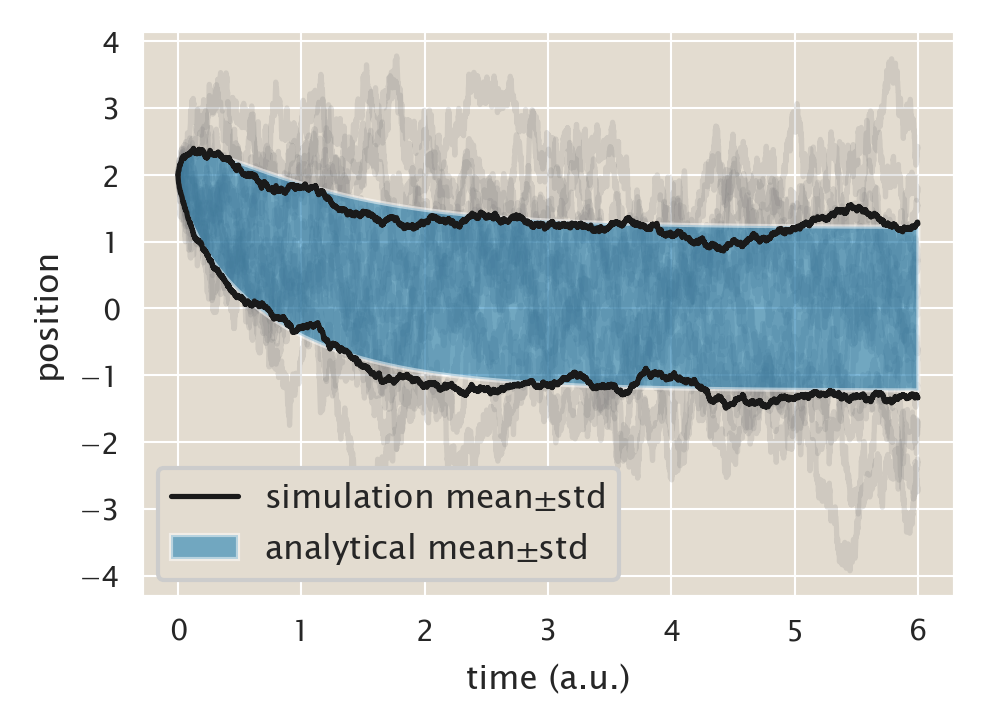
\includegraphics[width=0.5\textwidth]
  {../fig/drift_langevin/02_02_03_langevin_euler.png}
	\caption{\textbf{Numerical integration of the Langevin equation}. Comparison of simulation-based results with analytical results. Random trajectories that evolve according to \eref{eq_random_walk_langevin} were generated. From these the mean and standard deviation of the trajectories were computed (black lines). Analytical results for the mean $\pm$ standard deviation are shown as shaded blue area. For these simulations $x_o= 2$, $\gamma = 1$, $D = 1.5$, and $\Dt = 0.001$}
  \label{fig02_02_03}
\end{figure}

Having introduced the concept of random processes and the simple but yet
powerful Langevin equation our goal will now be to work out the mathematical
description of the full time evolution of the probability distribution of
possible realizations of the random process $P(x, t)$. Our goal will be to
derive the famous partial differential equation known as the Fokker-Plank
equation that exactly describes this time evolution.
\subsubsection{Stochastic growth}

The example we just studied in the previous section hopefully gave us some
intuition for how to work with these Langevin equations. Now we are ready to
apply these stochastic equations to our evolutionary context. In particular our
objective is to model the stochasticity of cellular growth. At the cellular
scale that we have been thinking about for bacteria, what this means is that
not all bacteria divide synchronously at the exact same time. There is a
distribution of cell-cycle length that depends on things such as nutrient
availability and temperature. The result of this cell-to-cell variability in
cell-cycle length is that there is noise in the growth curves that must be
accounted for. But how large is this noise and what is its functional form? In
other words, what is the form of the $B(x, t)$ term in \eref{eq_langevin}?

When we learn about bacteria growth we are usually told the fact that bacteria 
grow exponentially. This is a natural consequence of assuming that all bacteria
grow and divide at the same rate. So in the first division we pass from 1 to 2
bacteria, then we go from 2 to 4 and so on. This leads to an exponential growth
of the population.

% Chapter 3. Classic diffusion theory
% % !TEX root = ../../main.tex
\section{Classic diffusion theory in population genetics}

The pioneers of the modern-synthesis of evolution established solid foundations
for how to understand the different forces at play that shape the structure of
evolving populations. But combining all of these forces into a single
description remained challenging. In other words, describing the outcome of an
evolutionary process that combined deterministic processes such as selection
and mutation with the stochasticity of evolution presented a challenging
mathematical puzzle. The first attempt to put everything together came from
Sewall Wright himself, but the achievement of formalizing the theory is often
associated with a remarkable Japanese population genetics by the name of Motoo
Kimura.

Kimura jump to fame when in 1968 he presented his \textit{Neutral theory of
molecular evolution}. In here Kimura argued that associating every biological
aspect to the outcome of a selection-driven process was too much of a naive
picture. We previously mentioned that Wright thought about genetic drift as an
important component of the evolutionary process, but in this 1968 paper Kimura
argued that it was \textit{the} dominant force in evolution.

But what really brings us here to study part of Kimura's scientific legacy is
his use of diffusion equations in the context of population genetics. What we
know now as Kimura's diffusion theory is nothing else than the application of
the mathematical tools developed for the study of physical diffusion of
particles to evolving populations. Diffusion is one of several transcendent
concepts in physics that demonstrate the power of universal concepts. The same
equation that describes how the concentration of a chemical species changes as
a function of space and time is used to describe how the temperature profile of
an object changes as a function of space and time as well. Furthermore, as we
will study in this section, the same mathematical language can describe
diffusion on an abstract space of allele frequency. So as Joe Blitzstein likes
to say: ``nouns change, but the verbs remain the same.''

The mathematical language to study diffusion theory, as with many other field
of science is the language of probability theory. As Jaynes' famous book title
suggested, \textit{probability theory is the logic of science}. It is through
this formal language that we can assess how likely are specific events to
happen. For example, later on we'll see that within the framework of diffusion
theory is possible to ask what is the probability of an allele being fixed in
the population given the evolutionary forces acting on it. In particular we are
interested in a type of probability object known as a Markov process that we
will now define.

\subsection{Markov processes}
Of particular interested for our endeavor are the specific mathematical objects
known as Markov processes. The Markovian property - named after Andrey Markov,
a famous Russian mathematician from the XIX century - can be stated as follows:
A Markov process is a type of stochastic process for which the transition
states only depends on the current state.

To gain intuition for what this means imagine we are measuring a variable $x$
over time such that we have a bunch of pairs of the form $(x_1, t_1), (x_2,
t_2), (x_3, t_3), \ldots (x_{n+1}, t_{n+1})$. For a Markov process, the
probability of ending at state $x_{n+1}$ at time $t_{n+1}$ given all the
previous visited states is of the form
\begin{equation}
  P(x_{n+1}, t_{n+1} \mid x_1, t_1; x_2, t_2; \ldots; x_n, t_n) =
  P(x_{n+1}, t_{n+1} \mid x_n, t_n).
  \label{eq_chapman_kolmogorov}
\end{equation}
In other words, knowing the entire history of variable $x$ as it evolves over
time does not help us predict the next time step. All we need to know is the
last position. Markov processes are usually called memoryless stochastic
process because of this property that the process doesn't remember the full
trajectory when it ``decides'' where to move in the next step. Assuming a
Markovian process is arguably one of the most widely used assumptions in all of
science; from chemical reactions, to brownian motion of a particle, to our
particular case of interest of allele frequencies changing over time.

In the classic formulation of diffusion theory we are concerned with a
particular type of Markov processes. Diffusion theory works in the limit of
large populations where we can assume that the frequency of a particular allele
rather than being a discrete entity that changes in factors of $1 / N$ where
$N$ is the number of organisms, is a continuous value in the range between 0
and 1. We also assume that we can compute changes in this frequency in
continuous time. That means that both $f$ the frequency of an allele, and $t$
the time are continuous variables. Therefore we are interested in a type of
Markov processes that go by the creative name of continuous-time
continuous-state Markov processes. We will now state a very important equation
for this type of Markovian processes known as the Chapman-Kolmogorov equation.

\subsubsection{Chapman-Kolmogorov equation} \label{sec_chapman_kolmogorov}

The Chapman-Kolmogorov equation is an important property of continuous-time
continuous-state Markov processes that we will use for many of our derivations
in the coming sections. The equation is stated as follows: For three time points
$t_1 < t_2 < t_3$ for which we measured a stochastic variable $x$ we have that
\begin{equation}
  P(x_3, t_3 \mid x_1, t_1) = \int dx_2\; P(x_3, t_3 \mid x_2, t_2)
                                          P(x_2, t_2 \mid x_1, t_1),
\end{equation}
where the integral is taken over the domain of values that the random variable
$x$ can take. In other words, to calculate the transition probability between
$x_1$ and $x_3$ with an intermediary step $x_2$, we must add (integrate for
continuous variables) all possible values that $x_2$ can take. This concept is
schematically represented in \fref{fig_03_02_01}

\begin{figure}[h!]
	\centering 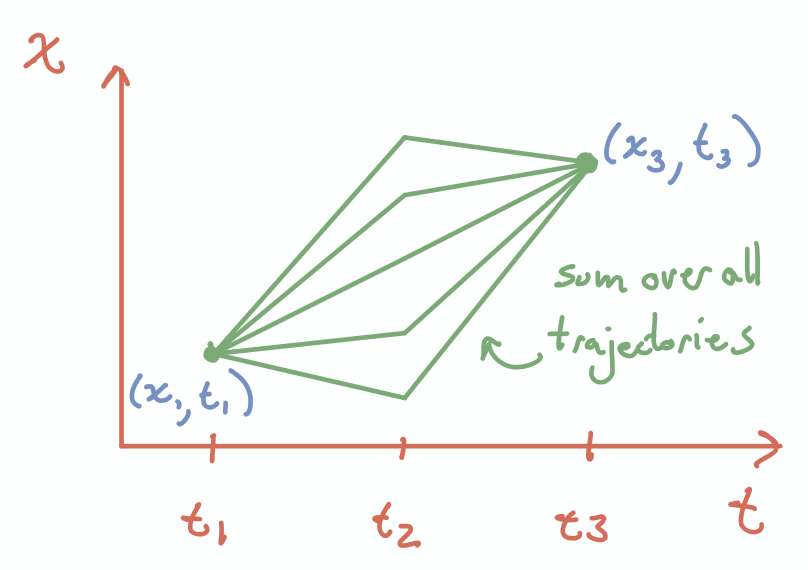
\includegraphics[width=0.5\textwidth]
  {../fig/classic_diffusion/03_02_01_chapman_kolmogorov.png}
	\caption{\textbf{Schematic of the Chapman-Kolmogorov equation}. The
  Chapman-Kolmogorov equation is a statement about the transition between two
  points $x_1$ and $x_3$, adding all possible intermediary steps $x_2$.}
  \label{fig_03_02_01}
\end{figure}

In the coming section we will use the Chapman-Kolmogorov equation to derive the
so-called continuous master equation. This will be the foundation from which we
will get to the main results of diffusion theory. But before jumping into such
matter we need to introduce a specific subtype of Markov processes.

\subsubsection{Stationary Markov Process}\label{sec_stationary_process}

When thinking about evolution we often summon the concept of a mapping between
genotype (sequence level description) to phenotype (observable characteristic)
to fitness (reproductive success). This concept goes by several names, but in
1932 Sewall Wright attempted to formalize this idea as \textit{adaptive
landscapes}. The phenotype itself can be a function of the genotype and the
environmental state that can itself change over time either deterministically
or stochastically. Therefore the idea of a ``landscape'' is not necessarily the
best description. Some authors have discussed concepts such as \textit{fitness
seascapes} when the environment evolves over time independently of the organism
or \textit{fitness snowscapes} when there is a direct interaction between
organisms modifying the environment, and the environment modifying the
organisms.

For simplicity we usually work with fixed fitness landscapes. This
approximation is valid under certain time-scale regimes. For example, if the
environment does change over time, but it does it on a time-scale much longer
than what it takes for organisms to adapt, then we can pretend for our
calculations that the environment is fixed, simplifying the math enormously.
For this particular case where the mapping all the way from genotype to fitness
is not a function of time is described by a type of stochastic chain known as
\textbf{stationary Markov process}. The formal definition of a stationary
Markov process can be stated as: A stationary Markov process is a memoryless
process for which when computing the moments of the distribution, these are not
affected by a time shift $\tau$, i.e.
\begin{equation}
  \ee{X(t_1 + \tau) X(t_2 + \tau) \cdots X(t_n + \tau)} =
  \ee{X(t_1) X(t_2) \cdots X(t_n)}.
\end{equation}
In other words, for a stationary Markov process what matters are the absolute
time differences $|t_2 - t_1|$ rather than the absolute time points. This
implies that the probability of our random variable having a particular value
$x$ is governed by a probability distribution $P_X(x)$ with no time dependence.
Notice the difference between the statements: On the one hand if we want to
know what is the probability of the random variable transitioning from a value
$x$ to a value $x'$ all we need to know is how much time passed between both
instances of the random process. On the other hand if we are only interested in
knowing what is the probability of the random variable taking a specific value
there is no time dependence for a stationary process since this probability
will not change over time. For the evolution questions we will be addressing
here is easy to see how this implies a fixed adaptive landscape. Since the
environment is fixed the mapping between genotype all the way to fitness will
be the same regardless of the time at which the population acquires a specific
allele frequency.

Now we are ready to derive the master equation that will describe the time
evolution of the probability distribution of allele frequencies.
% \section{The (continuous) master equation for allele frequencies}

One of the most powerful tools to study stochastic process is the so-called
master equation. Originally devised to study the stochastic time evolution of
chemical reactions - thereby christened the chemical master equation - this
equation has found applications in many areas of chemistry, physics and biology.
The equation is as statement about the time evolution of the transition
probabilities of a Markov process. That is just a fancy way of saying that the
master equation describes how the transition probabilities between states change
over time.

Let's derive this powerful equation starting from \eref{eq_chapman_kolmogorov}.
For our case of study we want to understand how the frequency of a particular
allele evolves over time, that is a stochastic process $F(t)$. Notice again that
we distinguish between the stochastic process $F(t)$ formed by the ensemble of
all possible realizations $f(t)$. The Chapman-Kolmogorov equation for this
particular case with three time points $t_1 < t_2 < t_3$ takes the form
\begin{equation}
  P(f_3, t_3 \mid f_1, t_1) = \int_0^1 df_2\; P(f_3, t_3 \mid f_2, t_2)
                                          P(f_2, t_2 \mid f_1, t_1),
  \label{eq_chapman_freq}
\end{equation}
where the integration limits $[0, 1]$ are the domain of values that an allele
frequency can take. Now let us assume that we observe the frequency at time $t$
and it happens to be at a value $f_1$. Then after a very short time $\Dt$ we
observe again the allele frequency which is now at a value $f_2$. Under this
short time limit we can approximate the transition probability as
\begin{equation}
  P(f_2, t + \Dt \mid f_1, t) = \delta(f_2 - f_1)
  \underbrace{\left[ 1 - a^{(0)}(f_1, t) \Dt \right]}_{\text{probability
  of no transition}} +
  \underbrace{\phi_t(f_2 \mid f_1)\Dt}_\text{probability of transition} +
  \mathcal{O}(\Dt^2).
  \label{eq_transition_short_time}
\end{equation}
Let's break down this equation. We have split the possible things that can
happen on a time window $\Dt$ into two possible cases. The first one represented
by the first term on the right-hand side is the possibility that on this small
time window no transition actually takes place. The $\delta$-function that is
equal to 1 if and only if $f_2 = f_1$ is there to make sure that this term is
added only when there was no transition during that time and $f_2$ remains the
same as $f_1$. Inside the square brackets we wrote $1 - a^{(0)}(f_1, t) \Dt$,
the reason for writing the term $a^{(0)}$ will become clear later on when we
derive the so-called Fokker-Planck equation. Having a term of the form 1 -
``something'' hints at the fact that this ``something'' must be the probability
of transitioning somewhere else rather than staying at the same position. For
the second term we wrote $\phi_t(f_2 \mid f_1)\Dt$ as the probability of
transitioning outside of $f_1$ during this time window. our function $\phi_t(f_2
\mid f_1)$ represents the transition probability per unit time between $f_1$ and
$f_2$ at time $t$. When we multiply this rate in time$^{-1}$ units by a small
time window, we obtain the probability of transitioning from $f_1$ to $f_2$.

In order to understand better the term $a^{(0)}(f_1, t)$ in
\eref{eq_transition_short_time} recall that a probability distribution must be
normalized. That means that if we integrate both sides of
\eref{eq_transition_short_time} over all values of $f_2$ it must be true that
\begin{equation}
  \int_0^1 df_2 \; P(f_2, t + \Dt \mid f_1, t) =
  \int_0^1 df_2 \; \delta(f_2 - f_1) \left[ 1 - a^{(0)}(f_1, t) \Dt \right]
  + \int_0^1 df_2 \; \phi_t(f_2 \mid f_1)\Dt
  = 1.
\end{equation}
Integrating over the $\delta$-function implies that we set $f_2 = f_1$,
therefore we obtain
\begin{equation}
  1 = \left[  1 - a^{(0)}(f_1, t) \Dt\right] +
  \int_0^1 df_2 \; \phi_t(f_2 \mid f_1)\Dt.
\end{equation}
Solving for $a^{(0)}(f_1, t)$ results in
\begin{equation}
  a^{(0)}(f_1, t) = \int_0^1 df_2 \; \phi_t(f_2 \mid f_1),
  \label{eq_a0}
\end{equation}
proving our previous assertion that $a^{(0)}(f_1, t)$ must be the
probability of jumping from $f_1$ to somewhere else.

Using this approximation for short time steps we will now derive the
differential equation that the transition probability between frequencies must
obey. Specifically for three time points $t_o < t < t + \Dt$ with corresponding
allele frequencies $f_o, f', f$ we have that \eref{eq_chapman_freq} takes the
form
\begin{equation}
  P(f, t + \Dt \mid f_o, t_o) = \int_0^1 df' \; P(f, t + \Dt \mid f', t)
  P(f', t \mid f_o, t_o).
\end{equation}
Substituting \eref{eq_transition_short_time} results in
\begin{equation}
  P(f, t + \Dt \mid f_o, t_o) = \int_0^1 df' \;
  \left[ \delta(f - f') \left( 1 - a^{(0)}(f', t)\Dt \right)
  + \phi_t(f \mid f')\Dt \right]
  P(f', t \mid f_o, t_o).
\end{equation}
Evaluating the integral for the first term on the right-hand side gives
\begin{equation}
  P(f, t + \Dt \mid f_o, t_o) = \left[\left( 1 - a^{(0)}(f, t)\Dt \right)\right]
  P(f, t \mid f_o, t_o) +
  \Dt \int_0^1 df' \; \phi_t(f \mid f') P(f', t \mid f_o, t_o).
\end{equation}
We can then substitute \eref{eq_a0} and rearrange terms to obtain
\begin{equation}
  P(f, t + \Dt \mid f_o, t_o) = P(f, t \mid f_o, t_o)
  + \int_0^1 df' \left[ \phi_t(f \mid f') P(f', t \mid f_o, t_o) -
  \phi_t(f' \mid f) P(f, t \mid f_o, t_o) \right]\Dt.
\end{equation}
Sending the first term on the right-hand side to the left, dividing both sides
by $\Dt$ and taking the limit $\Dt \rightarrow 0$ gives the differential
equation we were looking for
\begin{equation}
  \dt{P(f, t \mid f_o, t_o)} = \int_0^1 df' \;
  \underbrace{
  \left[ \phi_t(f \mid f') P(f', t \mid f_o, t_o) \right.}
  _{\text{gain } f' \rightarrow f}  -
  \underbrace{
  \left. \phi_t(f' \mid f) P(f, t \mid f_o, t_o) \right]}
  _{\text{loss } f \rightarrow f'}.
  \label{eq_master_eq_trans}
\end{equation}
This is the integro-differential equation known as the master equation. This
continuous form of the master equation describes the time evolution of the
transition probabilities $P(f, t \mid f_o, t_o)$, not the evolution of the
probability of being at a specific state $P(f, t)$. However we can use the rules
of probability to obtain such description by the following process: Suppose the
stochastic process $F(t)$ describes the time evolution of the frequency.
Assuming $F(t)$ is a stationary Markov process as described in
\secref{sec_stationary_process} means that this process is completely
characterized by two functions - the probability of having a particular value
for the allele frequency $P_F(f)$ that does not depend on time, and a transition
probability $P(f, t \mid f_o, t_o)$. We define a new, non-stationary process
$F^*(t)$ for $t \geq t_o$ by setting
\begin{equation}
  P^*(f, t) = P(f, t\mid f_o, t_o),
\end{equation}
i.e. forcing the initial condition to be a specific value $f_o$ at time $t_o$.
This is a sub-ensemble of the process $F(t)$ since we demanded that $F(t = t_o)
= f_o$. More generally if instead of setting the initial condition to be a
single specific value $P(f, t_o) = \delta(f - f_o)$ we define a probability
distribution for the initial state $P(f, t_o) = \rho(f_o)$, we have a
sub-ensemble of the form
\begin{equation}
  P^*(f, t) = \int_0^1 df_o \; P(f, t\mid f_o, t_o) \rho(f_o).
  \label{eq_subensemble}
\end{equation}
The interpretation of this sub ensemble is that the system was initially set on
a non-stationary state. The initial state distribution $\rho(f_o)$ does not
depend on time, therefore if we take the time derivative on both sides of
\eref{eq_subensemble} we find that
\begin{equation}
  \dt{P^*(f, t)} = \int_0^1 df_o \; \dt{P(f, t\mid f_o, t_o)}
                        \rho(f_o).
\label{eq_subensemble_dt}
\end{equation}
Notice that the term with the time derivative on the right-hand side of
\eref{eq_subensemble_dt} is the master equation that we derived in
\eref{eq_master_eq_trans}. Substituting this results in
\begin{equation}
  \dt{P^*(f, t)} = \int_0^1 df_o \; \rho(f_o)
  \int_0^1 df' \;
  \left[ \phi_t(f \mid f') P(f', t \mid f_o, t_o) -
  \phi_t(f' \mid f) P(f, t \mid f_o, t_o) \right].
\end{equation}
Redistributing the integrals gives
\begin{equation}
  \dt{P^*(f, t)} = \int_0^1 df' \; \phi_t(f \mid f')
  \overbrace{
  \int_0^1 df_o \; P(f', t \mid f_o, t_o) \rho(f_o)}
  ^{P^*(f', t)\text{ by definition}} -
  \int_0^1 df' \; \phi_t(f' \mid f)
  \overbrace{
  \int_0^1 df_o \; P(f, t \mid f_o, t_o) \rho(f_o)}
  ^{P^*(f, t)\text{ by definition}}.
\end{equation}
Using the definition of the sub-ensembles shown in \eref{eq_subensemble} we
arrive to a result of the form
\begin{equation}
  \dt{P^*(f, t)} = \int_0^1 df' \;
  \underbrace{
  \phi_t(f \mid f') P^*(f', t)
  }_{f' \rightarrow f \text{ gain}} -
  \int_0^1 df' \;
  \underbrace{
  \phi_t(f' \mid f) P^*(f, t)
  }_{f \rightarrow f' \text{ loss}}.
  \label{eq_master_eq_full}
\end{equation}
In this form we can see that the master equation is a balance between gain and
loss of probability at each state $f$. Having said that, the truth about the
continuous master equation is that is extremely complicated to work with. In
general integro-differential equations are challenging mathematical objects to
deal with. That is why in the next section we'll use the powerful tool of
Taylor expansions to simplify the equation. But before that let's discuss some
historic uses of the master equation that might look different to our derivation
on \eref{eq_master_eq_full}.

\subsection{Einstein-Kimura continuous master equations}

In 1905 during the groundbreaking year of Einstein's scientific career he
published a paper in which he attempted to give a molecular explanation to the
phenomena of Brownian motion. For this he derived Fick's second law from of a
statistical argument by Taylor expanding a master equation - more on that in
the next section. In this classic paper Einstein had one of the very first uses
of a continuous master equation applied to a physical problem. The difference
from our approach is that Einstein didn't derive the master equation from the
Chapman-Kolmogorov property of continuous-time continuous-state Markov
processes, but simply proposed its functional form directly.

While the problem Einstein was addressing in his paper had to do with a random
walker moving in real space, the mathematical tools that he proposed can be
directly mapped to the population genetics setup. As a matter of fact Motoo
Kimura himself used an equivalent approach to Einstein's formulation of the
master equation for his formulation of diffusion theory. Kimura used the same
approach as Einstein of Taylor expanding the master equation, with the main
difference being that for population genetics the transition probability
$\phi_t(f \mid f')$ is a function of the current position $f'$ while in real
space free diffusion is independent of the position. For this short section our
objective is to show that our derivation of the master equation is equivalent to
Einstein's and Kimura's proposed functional form. We will focus on Kimura's
version of the master equation since population genetics is what concerns us in
these notes.

Kimura's original derivation of the classic diffusion theory begins stating that
the process of allele frequency changes can be stated as
\begin{equation}
  P(f, t + \Dt) = \int d\varepsilon \;
  P(f - \varepsilon, t) \phi_t(f \mid f - \varepsilon) \Dt,
  \label{eq_kimura_master}
\end{equation}
and that is it. While it took us a while to justify \eref{eq_master_eq_full},
Kimura (and Einstein in the context of Brownian motion) simply stated the master
equation as the starting point. There is nothing intrinsically wrong about
having \eref{eq_kimura_master} as the starting point, but in this set of extend
notes I thought it would be insightful to start from a more fundamental property
of Markov processes and have the master equation be a consequence of such
property. Also I would like to highlight that in all of the population genetics
literature I have come across so far there has never been an explicit account of
the integration limits on the equations. This includes Kimura's original work as
well as textbooks. For this particular case the integration limits should go
from $f$ to $f - 1$ such that the values of $f - \varepsilon$ range from 0 to 1.
So the proper form of this integral is given by
\begin{equation}
  P(f, t + \Dt) = \int_{-f}^{f - 1} d\varepsilon \;
  P(f - \varepsilon, t) \phi_t(f \mid f - \varepsilon) \Dt.
  \label{eq_kimura_master_lim}
\end{equation}

Notice that at first glance \eref{eq_master_eq_full} and
\eref{eq_kimura_master_lim} don't seem to be equivalent.
\eref{eq_master_eq_full} is a differential equation that describes how the
probability distribution changes given gains and losses of probability on state
$f$, while \eref{eq_kimura_master_lim} only makes a statement of what would the
probability distribution look like a tiny time step into the future by adding
all the jumps \textbf{into} state $f$, but it doesn't include a term for all the
jumps out of state $f$. To show that these equations are equivalent we have to
do two things:
\begin{enumerate}
  \item On \eref{eq_master_eq_full} we notice that the second term on the
  right-hand side can be written as
  \begin{equation}
    P^*(f, t)\int_0^1 df' \; \phi_t(f' \mid f) = P^*(f, t),
    \label{eq_integral_transition}
  \end{equation}
  where we took the term $P^*(f, t)$ outside of the integral and used the fact
  that the transition probability per unit time $\phi_t(f' \mid f)$ should be
  normalized regardless of the time window. In other words, the probability of
  transitioning from $f$ to anywhere else (including staying at $f$) should add
  up to one regardless of the time window we observe.
  \mrm{Need to check this statement and that the units make sense}
  \item Having this result we can rewrite \eref{eq_master_eq_full} as
  \begin{equation}
    \dt{P^*(f, t)} = \int_0^1 df' \;
    \phi_t(f \mid f') P^*(f', t) - P^*(f, t).
    \label{eq_master_eq_rearange}
  \end{equation}
  We are almost there! All is left is to notice that if we were to Taylor expand
  the left-hand side of \eref{eq_kimura_master_lim} with respect to time up to
  first order (as it is often done for time derivatives) we would obtain
  \begin{equation}
    P(f, t + \Dt) = P(f, t) + \dt{P(f, t)}\Dt + \mathcal{O}(\Dt^2).
  \end{equation}
  That means we can send the second term on the the right-hand side of
  \eref{eq_master_eq_rearange} to the left and rewrite the equation as
  \begin{equation}
    {P^*(f, t + \Dt) \over \Dt} = \int_0^1 df' \;
    \phi_t(f \mid f') P^*(f', t),
  \end{equation}
  which is equivalent to \eref{eq_kimura_master_lim} where instead of having
  the integration over the jump size $\varepsilon$ the integration is done over
  the final position $f'$.
\end{enumerate}

% % !TEX root = ../../main.tex
\section{Kramers-Moyal expansion of the Master equation}

For the most part master equations are hard to deal with beacause of their
integro-differential nature. A way around this issue is to simplify the master
equation using Taylor expansions. This expansion goes by name of Kramers-Moyal
expansion, and the truncated version of the expansion is known in physics
literature as the Fokker-Planck equation, and in the probability theory
literature as the Kolmogorov forward equation. Regardless of the fancy names
behind these manipulations the idea is very straight-forward and very common in
physics in general: we take a complicated function and use its derivatives to
come up with an approximation that is good enough at least locally.

To perform the expansion we need to express the transition probabilities
$\phi_t(f \mid f')$ in \eref{eq_master_eq_full} as a function of the jump size
$r \equiv f - f'$ rather than as conditional probabilities. We therefore
express the transition probabilities as
\begin{equation}
  \phi_t(f \mid f') = \phi_t(f'; r).
  \label{eq_trans_jump_size}
\end{equation}
By performing this change of variables for the integral in
\eref{eq_master_eq_full} we need to compute the Jacobian which is of the form
\begin{equation}
  dr = df' {dr \over df'} = -df'.
\end{equation}

Furthermore since the integration now is done over values of $r$ rather than
$f'$ we must update the integration limits as well. We then have for the lower
limit $f' = 0$ that upon substitution on the definition of $r$ this gives
\begin{equation}
  r(f' = 0) = f - 0 = f.
\end{equation}
Doing the same for the upper limit of $f' = 1$ results in
\begin{equation}
  r(f' = 1) = f - 1.
\end{equation}
Using these changes results in a master equation of the form
\begin{equation}
  \dt{P(f, t)} = \int_f^{f - 1} \underbrace{(-1)}_{\text{Jacobian}} dr \;
  \left[
  \phi_t(f - r; r) P(f - r, t) -
  \phi_t(f; -r) P(f, t)
  \right].
\end{equation}
For the second term inside the square brackets we wrote $\phi_t(f; -r)$ due to
the change of reference point. Since the original term was $\phi_t(f' \mid f)$
that means that the jump took place from $f$ to $f'$ instead of the other way,
therefore the jump rather than being of size $r$ it must be of size $-r$ to
compensate for this change. Flipping the limits of integration because of the
negative sign that the Jacobian gave results in
\begin{equation}
  \dt{P(f, t)} = \int^f_{f - 1} dr \;
  \phi_t(f - r; r) P(f - r, t) -
  \int^f_{f - 1} dr \;
  \phi_t(f; -r) P(f, t).
  \label{eq_master_eq_jump}
\end{equation}
Having showed what the integration limits \textit{should look like} we come
back to the issue mentioned before. Nowhere in the literature I have come
across there has been an explicit account for these limits. From Kimura to Rice
to even Lassig, everyone seems to overlook what these integrations should be.
In an attempt to be more explicit and thorough, while still readable and
intuitive I wanted to show the limits for the integral in the master equation.
Nevertheless these limits will have to be modify for our approximations as we
will see in a bit.

As mentioned before, dealing with \eref{eq_master_eq_jump} is extremely
complicated due to its integro-differential nature. To simplify things now we
will make use of one of the most handful techniques ever given to physics - the
Taylor expansion. This expansion will allow us to cast the nasty
integro-differential equation into a partial differential equation of infinite
order. This again is difficult to deal with, but we can always compromise some
precision for simplicity by truncating the expansion up to some arbitrary order
that is easier to handle. In particular is common practice to truncate
expansions up to second order, giving in this case one of Motoo Kimura's most
fundamental results, and the basis of all of diffusion theory in population
genetics. To perform the expansion of the master equation we have to assume the
following:
\begin{itemize}
  \item Changes on $f$ occur via very small jumps; i.e. the transition
  probability $\phi_t(f; r)$ is sharply peaked as a function of $r$, but at the
  same time varies slowly enough with $f$. This is a reasonable assumption in
  the limit of large population sizes since changes in the allele frequency
  will be slow for this regime.
  \item The probability of an allele frequency $P(f, t)$ also varies slowly
  with $f$. This smoothness requirement for the distribution is necessary since
  the expansion requires computing derivatives.
\end{itemize}
Both of these assumptions are necessary for the expansion to be valid at least
locally around the point we expand at.

\subsection{Issues with the integration limits}

As mentioned before, the integration limits on \eref{eq_master_eq_jump} must be
modified if we want to perform the Kramers-Moyal expansion. To show why this is
the case we will first attempt the expansion keeping the limits. Given the
assumptions we listed we can expand the first integrand in
\eref{eq_master_eq_jump} in powers of $f$ obtaining
\begin{equation}
  \begin{split}
    \ddt{P(f, t)} &= \int^f_{f - 1} dr \;
    \left[
    \phi_t(f; r) P(f, t) -
    {\partial \over \partial f} \left( \phi_t(f; r) P(f, t) \right) r \right. \\
    &+ \left.
    {1 \over 2} {\partial^2 \over \partial f^2}
    \left( \phi_t(f; r) P(f, t) \right) r^2 -
    {1 \over 3!} {\partial^3 \over \partial f^3}
    \left( \phi_t(f; r) P(f, t) \right) r^3 + \ldots
    \right] \\
    &-
    P(f, t) \int_{f - 1}^f dr \; \phi_t(f, -r).
  \end{split}
\end{equation}
If we now distribute the integral and write the general form of the expansion
we obtain
\begin{equation}
  \begin{split}
    \ddt{P(f, t)} &= P(f, t)\int^f_{f - 1} dr \; \phi_t(f; r) \\
    &+
    \sum_{k=1}^\infty {(-1)^k \over k!} {\partial^k \over \partial f^k}
    \left[
    P(f, t) \int_{f-1}^f dr \; r^k \phi_t(f; r)
    \right] \\
    &-
    P(f, t) \int_{f - 1}^f dr \; \phi_t(f, -r).
  \end{split}
\end{equation}
The problem with this expansion is that all integrals of the form
\begin{equation}
  \Phi(f, k) = \int_{f-1}^f dr \; r^k \phi_t(f; r),
  \text{ for } k \in \mathbb{N},
\end{equation}
have the wrong integration limits. Recall that we set these limits to cover the
entire domain of values that the jump size could take. Before the expansion
these limits allowed $\phi_t(f - r; r)$ to cover all jumps from any point
between zero and one towards $f$; after the expansion this is not true anymore.
For example if we were to substitute the lower integration limit into the
transition probability $\phi_t(f; r = f-1)$, the resulting final position $f +
f -1 = 2f -1$ would be outside of the range $[0, 1]$ for all $f < 1$. That is
why the Kramers-Moyal expansion is generally done for cases in which the
boundaries are irrelevant, for example Einstein's Brownian motion problem
didn't have this issue since the integration was taken from $-\infty$ to
$\infty$.

So how do we overcome this issue? The way to overcome this difficulty is to
set the integration limits to some irrelevant boundary. But in order to do so
we need to define our transition probability $\phi_t(f; r)$ to be zero if the
jump falls outside of the range $[0, 1]$. In other words, we could define the
transition probability as a piecewise function
\begin{equation}
  \phi_t(f; r) =
  \begin{cases}
    \phi_t(f + r \mid f)& \text{for } (f + r), f \in [0, 1] \\
    0& \text{otherwise}
  \end{cases}.
\end{equation}
This definition allow us to send the integration limits of
\eref{eq_master_eq_jump} from $-\infty$ to $\infty$ to still cover all possible
jumps. With this definition we then have
\begin{equation}
  \begin{split}
    \ddt{P(f, t)} &= P(f, t)\int^\infty_{- \infty} dr \; \phi_t(f; r) \\
    &+
    \sum_{k=1}^\infty {(-1)^k \over k!} {\partial^k \over \partial f^k}
    \left[
    P(f, t) \int_{-\infty}^\infty dr \; r^k \phi_t(f; r)
    \right] \\
    &-
    P(f, t) \int_{-\infty}^\infty dr \; \phi_t(f, -r).
  \end{split}
\end{equation}
Notice that the first and third term on the right-hand side of the equation are
integrating the transition probability over all possible jumps. Because of the
change of integration limits we proposed, these two terms cancel each other and
we are left with
\begin{equation}
  \ddt{P(f, t)} = \sum_{k=1}^\infty {(-1)^k \over k!}
  {\partial^k \over \partial f^k}
  \left[
  P(f, t) \int_{-\infty}^\infty dr \; r^k \phi_t(f; r)
  \right].
  \label{eq_almost_km}
\end{equation}
Let us now define the moments of the jump size distribution $\phi_t(f; r)$ to
be
\begin{equation}
  a^{(k)}(f, t) \equiv \int_{-\infty}^\infty dr \; r^k \phi_t(f; r),
  \label{eq_jump_mom}
\end{equation}
Then we can substitute this into \eref{eq_almost_km} to finally obtain the
Kramers-Moyal expansion of the master equation
\begin{equation}
  \ddt{P(f, t)} = \sum_{k=1}^\infty {(-1)^k \over k!}
  {\partial^k \over \partial f^k}
  \left[
  P(f, t) a^{(k)}(f, t)
  \right].
  \label{eq_km_expansion}
\end{equation}
Notice that on \eref{eq_transition_short_time} we used already the zero$\tth$
moment of the distribution; that's why the use of the notation $a^{(0)}(f, t)$.

So far we converted the complicated integro-differential form of the master
equation in \eref{eq_master_eq_jump} into an equally difficult partial
differential equation of infinite order. Therefore our ability to handle the
equation hasn't been simplified. In the next section we will deal with how to
actually improve our chances of making sense of this by truncating the
expansion up to second order.

% % !TEX root = ../../main.tex
\subsection{xokker-Planck equation in population genetics}

In the last section after we performed a Taylor expansion of the master
equation we ended up with an equally complicated partial differential equation
of infinite order. So in order to make any progress towards simplifying the
treatment of the equation what we will do is trade accuracy for simplicity.
More concretely if our assumptions on the shape of the transition probability
$\phi_t(x; r)$ being sharply peaked are to be taken seriously, we can then
truncate the Kramers-Moyal expansion to include only up to second order
derivatives. This truncated equation would locally approximate the time
evolution of the probability distribution $P(x, t)$. \eref{eq_km_expansion}
then is of the form
\begin{equation}
  \ddt{P(x, t)} = - {\partial \over \partial x}
  \left[
  a^{(1)}(x, t) P(x, t)
  \right] +
  {1 \over 2}{\partial^2 \over \partial f^2}
  \left[
  a^{(2)}(x, t) P(x, t)
  \right].
  \label{eq_fokker_planck}
\end{equation}
In the physics literature this is known as the Fokker-Planck equation, while in
the mathematics literature is known as the Kolmogorov forward equation. One
intriguing aspect of how to arrive to this equation is the seemingly arbitrary
choice of truncating up to the second moment. The argument that is often thrown
around is that the ``art'' of these truncations is to stop at the first
non-vanishing moment. But for the specific case of the Kramers-Moyal expansion
of the master equation there is a theorem - Pawula theorem - that shows that
for the solutions of the Kramers-Moyal expansion to be interpreted as
probability densities the expansion must either contain one, two or an infinite
number of moments. So two sounds much better than infinite, doesn't it?
\mrm{Need to include appendix with the proof of Pawula theorem.}

\subsubsection{Determination of the Fokker-Planck coefficients}

The two jump moments in \eref{eq_fokker_planck}, $a^{(1)}$ and $a^{(2)}$
defined by \eref{eq_jump_mom} have a specific interpretation in population
genetics. Here is where a little bit of a terminology conflict between physics
and evolutionary biology comes into play. The directional term, i.e. the one
with the first order derivative in \eref{eq_fokker_planck} is known in the
physics literature as the drift term on a diffusion-like equation. This is
confusing because in evolutionary theory the diffusive term, i.e. the one with
the second derivative in \eref{eq_fokker_planck} is known as the genetic drift
term. I will try to be as consistent as possible on these notes using the terms
directional and diffusive to avoid confusion.

Coming back to the directional term, we define $M(x, t)$ to be
\begin{equation}
  M(x, t) \equiv \ee{r(t)} = \int_{-\infty}^{\infty} dr \; \phi_t(x; r) r,
\end{equation}
i.e. the mean of the jump distribution. As we will see in coming sections this
term captures the effect of directional evolutionary forces such as selection,
mutation and migration. For the diffusive term we define $V(x, t)$ as the
second moment of the jump distribution
\begin{equation}
  V(x, t) \equiv \ee{r^2(t)} = \int_{-\infty}^{\infty} dr \; \phi_t(x; r) r^2.
\end{equation}
This term captures the random sampling of alleles, also known as genetic drift.
In all of the population genetics literature I have encounter so far, this term
$V(x, t)$ is treated as the \textbf{variance} rather than the second moment.
This is partly because computing the specific functional form of the variance
for different models of reproduction is much simpler. The variance
$\sigma_r^2(t)$ is defined as
\begin{equation}
  \sigma_r^2(t) = \ee{\left( r - \ee{r} \right)^2} = \ee{r^2} - \ee{r}^2.
\end{equation}
We can therefore work with this more convenient quantity if we assume that
$\ee{r}^2 \approx 0$. This is a reasonable assumption given that for the
Fokker-Planck equation to be accurate we assumed a tight distribution for the
jumpt size $\phi_t(x; r)$. The peaked nature of this distribution must imply
that $\ee{r} \ll 1$, but more importantly, we will assume that
$\ee{r}^2 \ll \ee{r^2}$. So upon using these two definitions we arrive to one
of the main results in population genetics, the Kimura diffusion equation
\begin{equation}
  \ddt{P(x, t)} = - {\partial \over \partial x}
  \left[
  M(x, t) P(x, t)
  \right] +
  {1 \over 2}{\partial^2 \over \partial f^2}
  \left[
  V(x, t) P(x, t)
  \right].
  \label{eq_kimura_diffusion}
\end{equation}
The power of diffusion theory is that in these two terms $M(x, t)$ and $V(x,
t)$ we can include all evolutionary forces acting simultaneously. The
functional forms of these specific terms depend on the reproduction model used.
We will explore that more specifically later on.

\subsubsection{Equilibrium distribution}

In the limit when $t \rightarrow \infty$ we expect the distribution of allele
frequencies to reach a steady-state $P_{ss}(x)$. For the 1D case we have
studied so far, i.e. two alleles with frequencies $x$ and $1 - x$ this steady
state is equivalent to an equilibrium distribution since detailed balance has
to be satisfied. To emphasize this point let us rewrite
\eref{eq_kimura_diffusion} as a statement of conservation of probability. This
is
\begin{equation}
  \ddt{P(x, t)} = - {\partial J(x, t) \over \partial x},
\end{equation}
where $J(x, t)$ is the probability flux at point $x$. If we set the time
derivative to zero there are only two options (in reality there is only one
option for 1D systems):
\begin{enumerate}
  \item ${\partial J \over \partial x} = 0; \; J \neq 0 \Rightarrow$ Steady
  state on a rotating or non-conservative field.
  \item ${\partial J \over \partial x} = 0; \; J = 0 \Rightarrow$ Equilibrium
  distribution that satisfies detailed balance.
\end{enumerate}
For our one-locus two-alleles case the second of these cases must be true.
What this implies is that at steady state the flux $J_{ss}(x)$ takes the form
\begin{equation}
  J_{ss}(x) = - M(x) P_{eq}(x) + {\partial \over \partial x}
  \left[ V(x) P_{eq}(x) \right] = 0,
  \label{eq_flux_eq}
\end{equation}
where we use $P_{eq}(x)$ to define that this is not only a steady-state
distribution, but an equilibrium distribution satisfying detailed balance.
\eref{eq_flux_eq} is a first order homogeneous ordinary differential equation.
We can solve it using the integration factor method. For this we define
$G(x) \equiv V(x)P_{eq}(x)$. Substituting this into \eref{eq_flux_eq} gives
\begin{equation}
  {- M(x) \over V(x)} G(x) + {\partial \over \partial x} G(x) = 0.
  \label{eq_ode_ss}
\end{equation}
In this form we define the integration factor to be
\begin{equation}
  h(x) = \exp \left( \int_0^x -{M(x') \over V(x')} \; dx' \right).
\end{equation}
Notice that we chose the limits of integration to be $[0, x]$. This is because
the fundamental theorem of calculus states that for any function $f(x)$ defined
in $[a, b]$, the antiderivative $F(x)$ is defined as
\begin{equation}
  F(x) = \int_a^x f(x') \; dx',
\end{equation}
regardless of the lower limit of integration. Multiplying both sides of
\eref{eq_ode_ss} by the integration factor $h(x)$ results in
\begin{equation}
  {- M(x) \over V(x)} G(x)
  \exp \left( \int_0^x -{M(x') \over V(x')} \; dx' \right)
  + {\partial \over \partial x} G(x)
  \exp \left( \int_0^x -{M(x') \over V(x')} \; dx' \right)
  = 0.
  \label{eq_ode_int_fact}
\end{equation}
The specific form of the integration factor was chosen such that we could
rewrite \eref{eq_ode_int_fact} as
\begin{equation}
  {d \over dx}
  \left[
  \exp \left(
  - \int_0^x {M(x') \over V(x')}
  \right)G(x) \; dx'
  \right] = 0.
\end{equation}
Written in this form we can simply integrate both sides with respect to $x$ as
\begin{equation}
  \int_0^x {d \over dx''}\left[
  \exp \left(
  - \int_0^{x''} {M(x') \over V(x')}
  \right) G(x'')\; dx'
  \right] =
  \int_0^x 0 \; dx''
\end{equation}
Evaluating these integrals results in
\begin{equation}
  \exp \left(
  - \int_0^{x} {M(x') \over V(x')}
  \right) G(x)\; dx' = C,
\end{equation}
where $C$ is an integration constant. Notice that for a specific interval
$[a, b] \in \mathbb{R}$ the integral of zero is
\begin{equation}
  \int_a^b 0 dt = 0,
\end{equation}
but when we set the upper integration limit as an independent variable, what we
are asking for is the antiderivative of zero which is a constant $C$.
Substituting the definition of $G(x) = V(x) P_{eq}(x)$ gives
\begin{equation}
  \exp \left(
  - \int_0^x dx' \; {M(x') \over V(x')}\right)
  V(x) P_{eq}(x) = C.
\end{equation}
We can then solve for the equilibrium allele distribution $P_{eq}(x)$ obtaining
the result we were aiming for
\begin{equation}
  P_{eq}(x) = {C \over V(x)} \exp \left(
  \int_0^x dx' \; {M(x) \over V(x)}
  \right).
\end{equation}
This is a Boltzmann-like distribution! The analogy with statistical mechanics
becomes even more clear when we substitute specific functional forms for the
directional term $M(x)$ and the diffusive term $V(x)$.

In the next section we will explore how to obtain the coefficients for our
Fokker-Planck equation given the Langevin dynamics that we defined in
\secref{sec_langevin_intro}.
% \subsection{From Langevin dynamics to Fokker-Planck equation}

Now that we built a description for the probability distribution over the
ensemble of trajectories that a Markovian stochastic process can follow we are
left with the task of how to define the Fokker-Plank equation coefficients from
the stochastic dynamics defined by the Langevin equation. Specifically in its
more general form we derived \eref{eq_fokker_planck} to depend on three things:
the probability distribution of allele frequencies $P(f, t)$, and the two jump
moments $a^{(1)}(f, t)$ and $a^{(2)}(f, t)$, where these moments are given by
\eref{eq_jump_mom}. A lot of the population genetics literature use a
non-mathematical argument to directly assign the values of these coefficients
given the either deterministic or stochastic nature of the terms. For example,
given the dynamics that we defined in \secref{seq_determ_mut} for the
deterministic form of mutation and selection (\eref{eq_sel_mut}) most texts
would directly assign these dynamics to be the first jump moment
$a^{(1)}(f,t)$. There is nothing intrinsically wrong with this approach, since
this is actually the correct answer, but it is not necessarily obvious that
this should be the case especially since \eref{eq_fokker_planck} requires us to
take a derivative with respect to $x$ of this coefficient multiplied by the
allele frequency distribution.

We will take a more formal approach and find how the terms in the Langevin
dynamics that we defined in \secref{sec_langevin_intro} connect to the
coefficients of the Fokker-Planck equation. To do so first we introduce a
quantity defined as
\begin{equation}
    \mathcal{A}^{(m)}(x; \tau, t) \equiv \int_{-\infty}^\infty dx\;
    (x - x')^m P(x, t + \tau \mid x', t), \; \text{for } m \geq 1.
    \label{eq_compute_jump_mom}
\end{equation}
This is nothing else than the average of $[x(t + \tau) - x(t)]^m$ with a sharp
initial condition $x(t) = x'$ for a Markov process that obeys the transition
probability distribution $P(x, t + \tau \mid x', t)$. Given that our Langevin
dynamics are Markov processes, the ensemble of trajectories must obey a
continuous master equation with such transition probability. Therefore
\eref{eq_compute_jump_mom} can be thought as the average displacement between
two time points $t$ and $t + \tau$ for our Langevin dynamics. In other words
$\mathcal{A}^{(m)}(x; \tau, t)$ can be expressed as
\begin{equation}
    \mathcal{A}^{(m)}(x; \tau, t) \equiv 
    \ee{\left[x(t + \tau) - x(t)\right]^m \mid x(t) = x'}.
    \label{eq_average_A}
\end{equation}
Just as we did to derive the master equation, for small $\tau$ we can rewrite
the conditional distribution $P(x, t + \tau \mid x', t)$ using
\eref{eq_transition_short_time}. Using this we can rewrite
\eref{eq_compute_jump_mom} as
\begin{equation}
    \mathcal{A}^{(m)}(x; \tau, t) = \int_{-\infty}^\infty dx\; (x - x')^m
    \underbrace{
    \left[ \delta(x - x') \left( 1 - a^{(0)}(x', t) \tau \right) +
    \phi_t(x \mid x')\tau \right]
    }_{P(x, t + \tau \mid x', t)}.
\end{equation}
Distributing the integrals results in
\begin{equation}
    \begin{aligned}
    \mathcal{A}^{(m)}(x; \tau, t) &= 
    \int_{-\infty}^\infty dx\; (x - x')^m \delta(x - x') \\
    &- \int_{-\infty}^\infty dx\; (x - x')^m \delta(x - x') a^{(0)}(x', t) 
    \tau \\ 
    &+ \int_{-\infty}^\infty dx\; (x - x')^m \phi_t(x \mid x') \tau.
    \end{aligned}
\end{equation}
For the first two terms we have that the $\delta$-function is one only when $x
= x'$ while the term $(x - x')^m$ is zero for this particular case. Therefore
both of these terms cancel and we are only left with
\begin{equation}
    \mathcal{A}^{(m)}(x; \tau, t) = \int_{-\infty}^\infty dx\; (x - x')^m 
    \phi_t(x \mid x') \tau.
\end{equation}
This is non other than the definition of the jump moments times $\tau$ given by
\eref{eq_jump_mom} since we defined $r \equiv x - x'$ and $\phi_t(x'; r) \equiv
\phi_t(x \mid x')$. Now we can see the connection; we started defining
$\mathcal{A}^{(m)}(x; \tau, t)$ to be the average displacement defined by our
Langevin dynamics over a small time interval $\tau$, and we found that this is
connected to the jump moments that define the coefficients of the Fokker-Planck
equation. So we have that
\begin{equation}
    \mathcal{A}^{(m)}(x; \tau, t) = \tau \cdot a^{(m)}(x, t).
\end{equation}
Given this result we can compute the jump moment by taking the derivative of
$\mathcal{A}^{(m)}$ with respect to $\tau$ and evaluating this derivative at
$\tau = 0$. This is
\begin{equation}
    a^{(m)}(x, t) = \left. {\partial \over \partial \tau} 
    \mathcal{A}^{(m)}(x; \tau, t) \right\vert_{\tau = 0}.
    \label{eq_A_tau_deriv}
\end{equation}
The reason we evaluate $\tau = 0$ is for convenience. In principle we could
evaluate the derivative for any value of $\tau$ since $a^{(m)}$ does not depend
on $\tau$, but zero is the one that simplifies things the most. Using the
definition of derivatives we then write \eref{eq_A_tau_deriv} as
\begin{equation}
    a^{(m)}(x, t) = \lim_{\Dt \rightarrow 0}
    \left.{\mathcal{A}^{(m)}(x, \tau + \Dt, t) - 
    \mathcal{A}^{(m)}(x, \tau, t) \over \Dt} \right\vert_{\tau = 0}.
\end{equation}
If we now substitute the equivalence of $\mathcal{A}^{(m)}$ with the average
displacement on our Langevin dynamics, i.e. \eref{eq_average_A} we obtain
\footnotesize
\begin{equation}
    a^{(m)}(x, t) = \lim_{\Dt \rightarrow 0} {1 \over \Dt}
    \left[
    \ee{\left[x(t + \tau + \Dt) - x(t)\right]^m \mid x(t) = x'} -
    \ee{\left[x(t + \tau) - x(t)\right]^m \mid x(t) = x'}
    \right]_{\tau = 0}.
    \label{eq_deriv_average}
\end{equation}
\normalsize
Now we use the condition $\tau = 0$ that we chose for simplification since the
second term in \eref{eq_deriv_average} cancels. We are then left with a simple
expression of the form
\begin{equation}
    a^{(m)}(x, t) = \lim_{\Dt \rightarrow 0}
    {\ee{\left[x(t + \Dt) - x(t)\right]^m \mid x(t) = x'} \over \Dt}.
\end{equation}
This result shows that given that our Langevin dynamics are a continuous Markov
process, we can compute the displacement dynamics for a small time interval,
elevate it to the $m\tth$ power, and then average it, to then compute the $m$
coefficient for the Fokker-Planck equation. Let's do this first for the first
coefficient $a^{(m)}(x, t)$.

\subsubsection{Directional coefficient of the Fokker-Planck equation}

For the first coefficient of the Fokker-Planck equation that defines the
directional terms of the dynamics we have
\begin{equation}
    a^{(1)}(x, t) = \lim_{\Dt \rightarrow 0}
    {\ee{x(t + \Dt) - x(t) \mid x(t) = x'} \over \Dt}.
\end{equation}
Recall that we defined the Langevin equations as a stochastic differential
equation given in \eref{eq_langevin}. Since $x(t)$ is the solution to this
differential equation we can use the fundamental theorem of calculus to rewrite
the average displacement as
\begin{equation}
    \ee{x(t + \Dt) - x(t) \mid x(t) = x'} =
    \ee{\left. \int_t^{t + \Dt} dt'\; {dx \over dt'} \right\vert x(t) = x'}.
\end{equation}
We then substitute \eref{eq_langevin} on the right-hand side to obtain
\begin{equation}
    \ee{x(t + \Dt) - x(t) \mid x(t) = x'} =
    \ee{\left.\int_t^{t + \Dt} dt'\; A(x, t') + B(x, t') \xi(t')\right\vert 
    x(t) = x'}.
\end{equation}
If we distribute the integral and use the linearity of expected values this
results in
\begin{equation}
    \ee{x(t + \Dt) - x(t) \mid x(t) = x'} =
    \int_t^{t + \Dt} dt\; A(x, t') + 
    \int_t^{t + \Dt} dt\; B(x, t') \ee{ \left.\xi(t') \right\vert x(t) = x'},
\end{equation}
where the only thing we needed to average over was the noise term $\xi(t)$. For
the Langevin equation we defined the average of this noise term to be zero
regardless of the initial position; that implies that the average displacement
is then simply given by
\begin{equation}
    \ee{x(t + \Dt) - x(t) \mid x(t) = x'} =
    \int_t^{t + \Dt} A(x, t').
\end{equation}
As a consequence the directional coefficient of the Langevin equation is then
of the form
\begin{equation}
    a^{(1)}(x, t) = \lim_{\Dt \rightarrow 0} {1 \over \Dt}
    \int_t^{t + \Dt} A(x, t').
\end{equation}
Since we are taking the limit when $\Dt \rightarrow 0$ we can approximate the
integral simply as
\begin{equation}
    a^{(1)}(x, t) \approx \lim_{\Dt \rightarrow 0}{1 \over \Dt} [A(x, t) \Dt] =
    A(x, t).
\end{equation}
We therefore mathematically justify the empirical argument commonly found in
the literature that the directional term associated with the Langevin equation
can be directly associated with the directional term of the Fokker-Planck
equation. In other words we showed that
\begin{equation}
    a^{(1)}(x, t) = A(x, t).
\end{equation}

\subsubsection{Diffusive coefficient of the Fokker-Planck equation}

To compute the second coefficient of the Fokker-Planck equation associated with
the diffusive random displacements we can follow the exact same recipe. First
we know that this coefficient is given by
\begin{equation}
    a^{(2)}(x, t) = \lim_{\Dt \rightarrow 0}
    {\ee{\left[x(t + \Dt) - x(t)\right]^2 \mid x(t) = x'} \over \Dt}.
\end{equation}
Again using the fundamental theorem of calculus gives us
\begin{equation}
    a^{(2)}(x, t) = \lim_{\Dt \rightarrow 0}
    {\ee{ \left. \left[ 
    \int_t^{t + \Dt} dt'\; {dx \over dt'}
    \right]^2 \right\vert x(t) = x'} \over \Dt}.
\end{equation}
Substituting \eref{eq_langevin} on the expected value on right-hand side gives
\begin{equation}
    \ee{ \left. \left[ 
    \int_t^{t + \Dt} dt'\; {dx \over dt'}
    \right]^2 \right\vert x(t) = x'} =
    \ee{ \left. \left[ 
    \int_t^{t + \Dt} dt'\; A(x, t') + 
    \int_t^{t + \Dt} dt'\; B(x, t') \xi(t').
    \right]^2 \right\vert x(t) = x'},
\end{equation}
where we already distributed the integral. We now expand the binomial on the
right-hand side and use the linearity of expected values to obtain
\begin{equation}
    \begin{aligned}
    \ee{ \left. \left[ 
    \int_t^{t + \Dt} dt'\; A(x, t') + 
    \int_t^{t + \Dt} dt'\; B(x, t') \xi(t')
    \right]^2 \right\vert x(t) = x'} =
    \left(  
    \int_t^{t + \Dt} dt'\; A(x, t')
    \right)^2\\
    + 2 
    \int_t^{t + \Dt} dt'\; A(x, t')
    \int_t^{t + \Dt} dt'\; B(x, t') \ee{ \left.\xi(t')
    \right\vert x(t) = x'}\\
    \left(
    \int_t^{t + \Dt} dt'\; B(x, t') \ee{\left.\xi(t')
    \right\vert x(t) = x'}
    \right)^2,
    \end{aligned}
\end{equation}
where again we used the fact that the only variable we can average over is the
white noise term $\xi(t)$.

    % \ee{\left.  \right\vert x(t) = x'}
% % !TEX root = ../../main.tex
\subsection{Kolmogorov backward equation}

So far with the Fokker-Planck equation we have been able to ask questions about
the entire distribution of allele frequencies accounting for the interplay of
different evolutionary forces simultaneously. Another interesting set of
questions has to do with asking what is the probability of the population
reaching a specific subset of states in a time $s > t$ given the current state
of the population $f(t)$. To be more specific we can ask what is the
probability of fixing an allele in a population as a function of its selective
advantage. For this kind of questions we use the so-called Kolmogorov-backward
equation. The name comes from the fact that compared to the forward equation,
i.e. the Fokker-Planck equation we derived in the previous section, we need to
integrate backwards in time.

The main difference between the forward and the backward equation has to do
with the emphasis on either the initial condition or the current state. As we
showed in \secref{sec_master_eq} the master equation is a statement about the
time evolution of the transition probability $P(f, t \mid f', t')$ for $t' \leq
t$. Let us set $f' \equiv f_o$, $t' \equiv t_o$ to be the initial conditions of
the random walker in allele frequency space. We then ask about the probability
of being at frequency $f$ at time $t$, i.e. $P(f, t + \Dt \mid f_o, t_o)$. This
probability is related to all of the possible paths that the variable $f$ can
take from the initial value $f_o$ at time $t_o$ to the value $f$ as shown
schematically in \fref{fig_03_05_01}.

\begin{figure}[h!]
	\centering 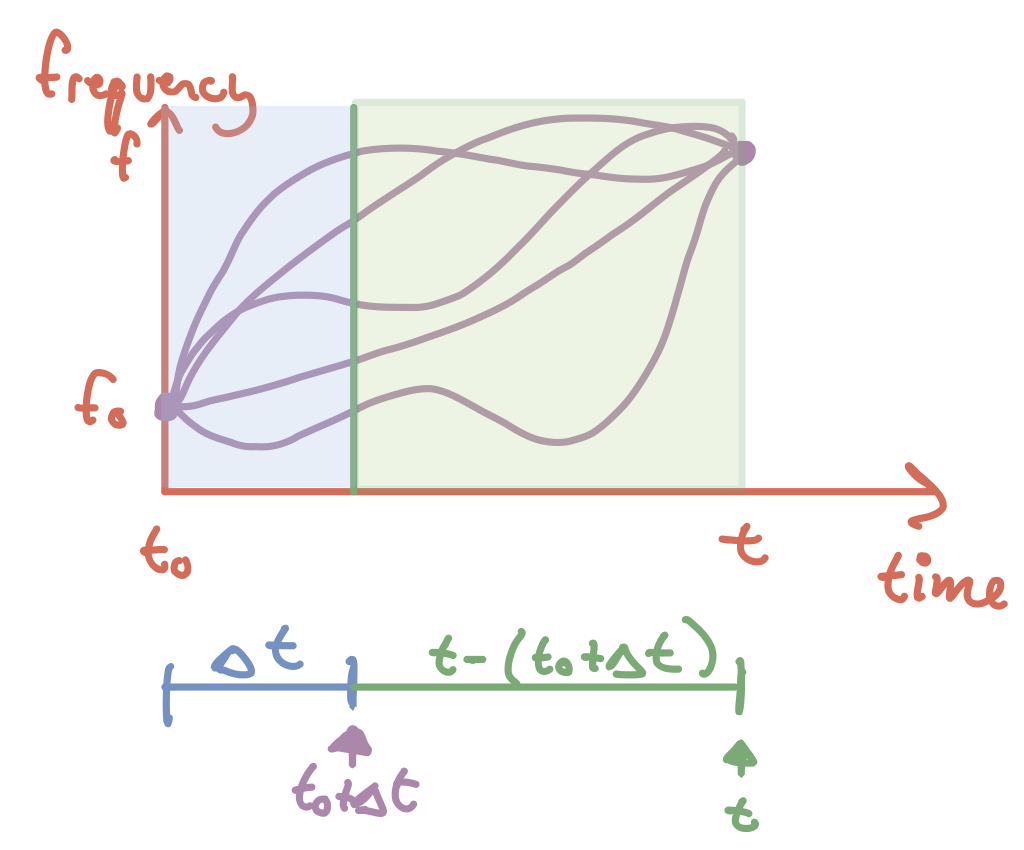
\includegraphics[width=0.5\textwidth]
  {../fig/classic_diffusion/03_05_01_schematic_reverse.png}
	\caption{\textbf{Schematic depiction of paths from $f_o$ to $f$}. The
	diagram shows schematically different paths that the allele frequency can
	take from an initial condition $f_o$ to a final point $f$ over a time $t$.
	The time is arbitrarily split into two intervals $[t_o, t_o + \Dt]$ shaded
	in blue and $[t_o + \Dt, t]$ shaded in green.}
  \label{fig_03_05_01}
\end{figure}

\subsubsection{Derivation of the Kolmogorov backward equation}

To derive the backward equation we can arbitrarily split the time interval in
two intervals $[t_o, t_o + \Dt]$ and $[t_o + \Dt, t]$. With this we can then
write down the Chapman-Kolmogorov equation that we stated in
\secref{sec_chapman_kolmogorov} as
\begin{equation}
  P(f, t \mid f_o, t_o) = \int_{-f_o}^{1 - f_o} dr \;
  P(f, t \mid f_o + r, t_o + \Dt)
  P(f_o + r, t_o + \Dt \mid f_o, t_o),
\end{equation}
where the limits of the integral on the right hand side were set such that the
quantity $f_o + r$ could cover the entire domain $[0, 1]$. For $\Dt$ very
small, specifically $\Dt \ll |t - t_o|$ we can write down the transition matrix
as we did for \eref{eq_transition_short_time}, obtaining
\begin{equation}
	P(f_o + r, t_o + \Dt \mid f_o, t_o) =
	\delta(r) \left[
	1 - a^{(0)}(f_o, t_o) \Dt
	\right] +
	\phi_{t_o}(f_o; r) \Dt,
\end{equation}
where $\phi_{t_o}(f_o; r) \Dt$ is the probability of taking a jumpt of size $r$
on a time window $\Dt$ given the initial position $f_o$ In this case the
$\delta$-function $\delta(r)$ is equal to one only when the jump $r$ is zero.
Notice that compared to the derivation of the forward equation where we first
wrote the corresponding master equation, here we start directly from the
transition distribution as a function of the jump size $r$. Substituting this
into the Chapman-Kolmogorov equation gives
\begin{equation}
	P(f, t \mid f_o, t_o) = \int_{-f_o}^{1 - f_o} dr\;
	P(f, t \mid f_o + r, t_o + \Dt)
	\left[
	\delta(r) \left( 1 - a^{(0)}(f_o, t_o) \Dt \right) +
	\phi_{t_o}(f_o; r) \Dt
	\right].
\end{equation}
If we distribute the integral and evaluate it over the delta function we obtain
\begin{equation}
	\begin{split}
		P(f, t \mid f_o, t_o) = P(f, t \mid f_o, t_o + \Dt)
		\left[
		1 - a^{(0)}(f_o, t_o)\Dt
		\right]\\ +
		\int_{-f_o}^{1 - f_o} dr\; P(f, t \mid f_o + r, t_o + \Dt)
		\phi_{t_o}(f_o; r) \Dt.
	\end{split}
	\label{eq_chap_kol_delta_eval_backwards}
\end{equation}
In \eref{eq_a0} we showed that $a^{(0)}(f_o, t_o)\Dt$ is the probability of
transitioning from $f_o$ to anywhere else. This is equivalent to writing
\begin{equation}
	a^{(0)}(f_o, t_o) \Dt \equiv \int_{-f_o}^{1 - f_o} dr \;
	\phi_{t_o}(f_o; r) \Dt.
\end{equation}
Substituting this result into \eref{eq_chap_kol_delta_eval_backwards} and
rearranging terms gives
\begin{equation}
	\begin{split}
	{P(f, t \mid f_o, t_o) - P(f, t \mid f_o, t_o + \Dt) \over \Dt} =
	- P(f, t \mid f_o, t_o + \Dt) \int_{-f_o}^{1 - f_o} dr \;
	\phi_{t_o}(f_o; r)\\
	+ \int_{-f_o}^{1 - f_o} dr \;
	P(f, t \mid f_o + r, t_o + \Dt) \phi_{t_o}(f_o; r).
	\end{split}
	\label{eq_almost_kolmogorov_backwards}
\end{equation}
If we assume our stochastic process is stationary (See
\secref{sec_stationary_process}), a perfectly reasonable assumption for a
fixed fitness landscape, it follows that
\begin{equation}
	 P(f, t + \tau \mid f_o, t_o + \tau) = P(f, t \mid f_o, t_o),
\end{equation}
for any $\tau$. In other words, for our stationary stochastic process what
matters is the time interval that happens between events rather than the actual
time. Using this we can then write the first term on the left-hand side of
\eref{eq_almost_kolmogorov_backwards} as
\begin{equation}
	P(f, t \mid f_o, t_o) = P(f, t + \Dt \mid f_o, t_o + \Dt).
\end{equation}
Using this time shift and taking the limit when $\Dt \rightarrow 0$ gives for
the left-hand side of \eref{eq_almost_kolmogorov_backwards}
\begin{equation}
	\lim_{\Dt \rightarrow 0} {P(f, t + \Dt \mid f_o, t_o + \Dt) -
	P(f, t \mid f_o, t_o + \Dt) \over \Dt} =
	\ddt{P(f, t \mid f_o, t_o)}.
\end{equation}
Using this for \eref{eq_almost_kolmogorov_backwards} results in
\begin{equation}
	\ddt{P(f, t \mid f_o, t_o)} =
	- P(f, t \mid f_o, t_o) \int_{- f_o}^{1 - f_o} dr \; \phi_{t_o}(f_o; r)
	+ \int_{- f_o}^{f_o} dr \; P(f, t \mid f_o + r, t_o) \phi_{t_o}(f_o; r).
\end{equation}
Notice we already took the limit $\Dt \rightarrow 0$ on both sides. We now
expand the second term on the right-hand side to obtain an analogous
Kramers-Moyal expansion for the Kolmogorov reverse equation. This is analogous
in the sense that we are not expanding a master equation as we did for the
forward equation. Also for this case we expand around the initial condition
$f_o$ rather than the final position $f$. Since the transition probability
$\phi_{t_o}(f_o; r)$ does not have a term $f_o + r$ it does not take part of
this expansion. Therefore we obtain
\begin{equation}
	\ddt{P(f, t \mid f_o, t_o)} =
	- P(f, t \mid f_o, t_o) \int_{- f_o}^{1 - f_o} dr \; \phi_{t_o}(f_o; r)
	+ \int_{-f_o}^{1 - f_o} dr\; \sum_{k=0}^{\infty} {1 \over k!}
	{\partial^k \over \partial f_o^k} P(f, t \mid f_o, t_o) r^k
	\phi_{t_o}(f_o; r).
\end{equation}
For this expansion we do not have issues with the integration limits. This
again happens because we are not expanding the master equation as we did for
the forward equation. The zero$\tth$ order term in the expansion cancels with
the first term on the right-hand side, obtaining
\begin{equation}
	\ddt{P(f, t \mid f_o, t_o)} =
	\sum_{k = 1}^{\infty} {1 \over k!} {\partial^k \over \partial f_o^k}
	P(f, t \mid f_o, t_o) \int_{-f_o}^{1 - f_o} dr\; \phi_{t_o}(f_o; r) r^k.
\end{equation}
We can again define the moments of the jump distribution $\phi_{t_o}(f_o; r)$
as
\begin{equation}
	a^{(k)}(f_o, t_o) \equiv \int_{-f_o}^{1 - f_o} dr \;
	r^k \phi_{t_o}(f_o; r).
\end{equation}
Using this we obtain the  expansion for the Kolmogorov backward equation
\begin{equation}
	\ddt{P(f, t \mid f_o, t_o)} =
	\sum_{k = 1}^{\infty} {1 \over k!} {\partial^k \over \partial f_o^k}
	P(f, t \mid f_o, t_o) a^{(k)}(f_o, t_o).
\end{equation}
Just as with the forward equation we can truncate the expansion up to second
order. Furthermore we define the first moments to be the mean jump size
\begin{equation}
	M(f_o) = \int_{-f_o}^{1 - f_o} dr \; r \phi_{t_o}(f_o; r).
\end{equation}
For small $M(f_o)$ we approximate the second moment as the variance
\begin{equation}
	V(f_o) \int_{-f_o}^{1 - f_o} dr \;
	(r - M(f_o))^2 \phi_{t_o}(f_o; r) \approx
	\int_{f_o}^{1 - f_o} dr \; r^2 \phi_{t_o}(f_o; r).
\end{equation}
Given these definitions we obtain the final form of the Kolmogorov backward
equation
\begin{equation}
	\ddt{P(f, t \mid f_o, t_o)} =
	M(f_o) {\partial \over \partial f_o}P(f, t \mid f_o, t_o) +
	{V(f_o) \over 2} {\partial^2 \over \partial f_o^2} P(f, t \mid f_o, t_o).
	\label{eq_kolmogorov_backward}
\end{equation}
This equation differs from the forward equation in several points:
\begin{itemize}
	\item The backward equation uses the conditional distribution with respect
	to the initial condition $P(f, t \mid f_o, t_o)$.
	\item The partial derivatives with respect to frequency are taken with
	respect to the initial condition $f_o$ as well.
	\item The jump moments are outside of the partial derivatives just as in a
	regular diffusion equation.
	\item There is no minus sign for the directional term.
\end{itemize}
As we will see in the following section the forward and backward equation
complement each other allowing us to tackle different questions. In particular
the backward equation can address the very interesting question of what is the
probability of an allele becoming fixed in the population.

\subsubsection{Equilibrium distribution of the Kolmogorov backward equation}

Rather than trying to solve directly this equation we can take the same
approach as we took for the forward equation and solve for the steady-state
distribution. For the case of the reverse equation the steady-state
distribution will tell us about in the very long time limit what is the
probability of ending at frequency $f$ given that the system started at a
frequency $f_o$. For example we can ask about the probability of an allele
going to fixation ($f = 1$) or extinction ($f = 0$) given some initial
frequency. To solve for the steady-state distribution first we set the time
derivative of \eref{eq_kolmogorov_backward} to zero
\begin{equation}
	0 = M(f_o) {\partial \over \partial f_o}P(f, t \mid f_o, t_o) +
	{V(f_o) \over 2} {\partial^2 \over \partial f_o^2} P(f, t \mid f_o, t_o).
	\label{eq_kolmogorov_backward_rev}
\end{equation}
We now define
\begin{equation}
	G(f_o) \equiv {\partial P(f, t \mid f_o, t_o) \over \partial f_o},
\end{equation}
and substitute this back on \eref{eq_kolmogorov_backward_rev}. With some
rearrangement of terms we obtain
\begin{equation}
	2 {M(f_o) \over V(f_o)} G(f_o) + {\partial G(f_o) \over \partial f_o} = 0.
\end{equation}
This is a first order linear ordinary differential equation that can be solved
using the integrating factor method just as we did for the equilibrium
distribution of the forward equation. For this we multiply both sides by
\begin{equation}
	h(f_o) = \exp \left( 2 \int_0^{f_0} df_o' {M(f_o') \over V(f_o')} \right),
\end{equation}
the integrating factor. This results in
\begin{equation}
	\exp \left( 2 \int_0^{f_0} df_o'\; {M(f_o') \over V(f_o')} \right)
	\left[
	2 {M(f_o) \over V(f_o)} G(f_o) + {\partial G(f_o) \over \partial f_o}
	\right] = 0.
\end{equation}
The integrating factor allows us to write this as
\begin{equation}
	{d \over df_o} \left[
	G(f_o) \exp \left(
	2 \int_0^{f_o} df_o' {M(f_o') \over V(f_o')}
	\right)
	\right] = 0.
\end{equation}
We can now integrate both sides with respect to $f_o$, obtaining
\begin{equation}
	\int_0^{f_o} df_o' \; {d \over df_o'} \left[
	G(f_o') \exp \left(
	2 \int_0^{f_o'} df_o'' \; {M(f_o'') \over V(f_o'')}
	\right)	\right] = \int_0^{f_o'} df_o' \; 0.
\end{equation}
Evaluating these integrals results in
\begin{equation}
	F(f_o) \exp \left(
	2 \int_0^{f_o} df_o' \; {M(f_o') \over V(f_o')}
	\right) = C,
\end{equation}
where $C$ is an integrating constant. If we now substitute back the definition
of $G(f_o)$ we obtain
\begin{equation}
	{\partial P(f, t \mid f_o, t_o) \over \partial f_o}
	\exp \left(
	2 \int_0^{f_o} df_o' \; {M(f_o') \over V(f_o')}
	\right) = C.
\end{equation}
We can use this equation to find the fixation probability of an allele.

\mrm{This again will be followed by specific cases on how to use this equation
to calculate fixation probabilities for different reproduction models.}




\end{document}
